% Template Tesi in Informatica, ispirata al template "Tesi di laurea - Universit� di Pisa" di Simone Schirinzi (https://www.overleaf.com/latex/templates/tesi-di-laurea-universita-di-pisa/rwdcqtqwftpg). 

% Carattere dimensione 12
\documentclass[12pt]{report}

% Per la stampa fronte-retro sostituire con:
% \documentclass[12pt, twoside]{report}

% Margini (4cm a sx, 2.5cm a dx, 2.5cm in alto, 2.5cm in basso)
\usepackage[top=2.5cm, bottom=2.5cm, left=4cm, right=2.5cm, centering]{geometry}

% Per la stampa fronte-retro sostituire con: 
% \usepackage[top=2.5cm, bottom=2.5cm, inner=4cm, outer=4cm, right=2.5cm, centering]{geometry}

% Interlinea
\linespread{1.5}

% Librerie utili
\usepackage[italian]{babel} % applicazione regole di scrittura per la lingua italiana 
\usepackage[utf8]{inputenc} % codifica UTF-8
\usepackage{scrlayer-scrpage} % stili pagina per il frontespizio
\ifoot[]{}
\cfoot[]{}
\ofoot[\pagemark]{\pagemark}
\pagestyle{scrplain}
\usepackage{mathptmx} % font Times New Roman (simile)
\usepackage{graphicx} % inserimento di immagini
\usepackage{csquotes} % per le citazioni "in blocco"
\usepackage{parskip}
\newcommand{\myenquote}[1]{``#1''}
%\usepackage[backend=biber, sorting=nty, ]{biblatex} % bibliografia con pacchetto biblatex (https://ctan.org/pkg/biblatex?lang=en)
\appto{\bibsetup}{\raggedright}

\usepackage{titlesec} % per la formattazione dei titoli delle sezioni, capitoli etc.
\usepackage{float} % per il posizionamento delle immagini

\usepackage{listings} % per il codice di programmazione
% Fonte https://en.wikibooks.org/wiki/LaTeX/Source_Code_Listings. Per la lista di sintassi riconosciute.
\renewcommand{\lstlistingname}{Codice}% Listing -> Codice
\usepackage{colortbl}
\usepackage{xcolor}  % stile del codice
\definecolor{mygreen}{rgb}{0,0.6,0}
\definecolor{mygray}{rgb}{0.5,0.5,0.5}
\definecolor{mymauve}{rgb}{0.58,0,0.82}
\definecolor{darkgray}{rgb}{.4,.4,.4}
\definecolor{navy}{HTML}{000080}
\definecolor{purple}{rgb}{0.65, 0.12, 0.82}
\definecolor{codepurple}{rgb}{0.58,0,0.82}
\definecolor{backcolour}{rgb}{0.95,0.95,0.92}

\definecolor{lightgray}{rgb}{0.9, 0.9, 0.9}
\usepackage{booktabs}
\usepackage{multirow}

% Stili configurabili del codice (lslisting) 
\lstset{ %
belowcaptionskip=0.5em,
backgroundcolor=\color{backcolour}, % choose the background color; you must add \usepackage{color} or \usepackage{xcolor}
basicstyle=\footnotesize, % the size of the fonts that are used for the code
breakatwhitespace=false, % sets if automatic breaks should only happen at whitespace
breaklines=true, % sets automatic line breaking
captionpos=b, % sets the caption-position to bottom
commentstyle=\color{mygreen}, % comment style
deletekeywords={...}, % if you want to delete keywords from the given language
escapeinside={\%*}{*)}, % if you want to add LaTeX within your code
extendedchars=true, % lets you use non-ASCII characters; for 8-bits encodings only, does not work with UTF-8
frame=single, % adds a frame around the code
keepspaces=true, % keeps spaces in text, useful for keeping indentation of code (possibly needs columns=flexible)
keywordstyle=\color{codepurple}, % keyword style
% language=Octave, % the language of the code
morekeywords={*,...}, % if you want to add more keywords to the set
numbers=left, % where to put the line-numbers; possible values are (none, left, right)
numbersep=5pt, % how far the line-numbers are from the code
numberstyle=\tiny\color{mygray}, % the style that is used for the line-numbers
rulecolor=\color{black}, % if not set, the frame-color may be changed on line-breaks within not-black text (e.g. comments (green here))
showspaces=false, % show spaces everywhere adding particular underscores; it overrides 'showstringspaces'
showstringspaces=false, % underline spaces within strings only
showtabs=false, % show tabs within strings adding particular underscores
stepnumber=1, % the step between two line-numbers. If it's 1, each line will be numbered
stringstyle=\color{mymauve}, % string literal style
tabsize=2, % sets default tabsize to 2 spaces
title=\lstname % show the filename of files included with \lstinputlisting; also try caption instead of title
}


% END of listing package 

% Esempio riconoscimento sintassi JavaScript 

\lstdefinelanguage{JavaScript}{
  keywords={typeof, new, true, false, catch, function, return, null, catch, switch, var, const, let, if, in, while, do, else, case, break},
  keywordstyle=\color{blue}\bfseries,
  ndkeywords={class, export, boolean, throw, implements, import, this},
  ndkeywordstyle=\color{darkgray}\bfseries,
  identifierstyle=\color{black},
  sensitive=false,
  comment=[l]{//},
  morecomment=[s]{/*}{*/},
  commentstyle=\color{mygreen}\ttfamily,
  stringstyle=\color{red}\ttfamily,
  morestring=[b]',
  morestring=[b]"
}

\lstset{
   language=JavaScript,
   extendedchars=true,
   basicstyle=\footnotesize\ttfamily,
   showstringspaces=false,
   showspaces=false,
   numbers=left,
   numberstyle=\footnotesize,
   numbersep=9pt,
   tabsize=2,
   breaklines=true,
   showtabs=false,
   captionpos=b
}

\usepackage{url}

% Formato delle intestazioni
\titleformat{\chapter}[block]
  {\normalfont\LARGE\bfseries}{\thechapter.}{0.5em}{\LARGE}
\titlespacing*{\chapter}{0pt}{-20pt}{25pt}

\begin{document}

% Frontespizio
\begin{titlepage}
\begin{figure}
    \centering
\includegraphics[scale=0.5]{immagini/cherubino_pant541.png}
\end{figure}

\begin{center}
    {\LARGE{ Dipartimento di Informatica \\}}
    \vspace{2cm}
    {\Large { TESI DI LAUREA }}\\
    \vspace{2cm}
    {\Large { Estensione di deployment Kubernetes per funzionalità di raccolta e analisi del logging in applicazioni a microservizi }}
\end{center}

\vspace{2cm}

\begin{minipage}[t]{0.47\textwidth}
	{\large{\bf Relatore:\\ Antonio Brogi}}
	\vspace{0.5cm}
	{\large{\bf \\Relatore:\\ Jacopo Soldani}}
\end{minipage}\hfill\begin{minipage}[t]{0.47\textwidth}\raggedleft
	{\large{\bf Candidato: \\ Giovanni Bellini\\ }}
\end{minipage}

\vspace{25mm}

\centering{\large{\bf ANNO ACCADEMICO 2022/2023 }}
\end{titlepage}
% Fine frontespizio
\begingroup
\pagestyle{empty}
\tableofcontents
\endgroup
\listoffigures

\thispagestyle{empty}
\clearpage
\addtocontents{toc}{\protect\thispagestyle{empty}}
\clearpage
\vspace*{\fill}
\thispagestyle{empty}

{\large \centering \textbf{Sommario} \par}

\vspace{1em} % Some space between title and abstract

% Justified text for the abstract
\noindent
Nell'ultimo decennio, è stato possibile assistere ad un'importante crescita nella diffusione delle applicazioni basate su microservizi. Questo perché strutturare un'applicazione a microservizi comporta svariati vantaggi, ma anche una maggiore complessità dell'architettura. Data questa maggiore complessità, l'abilità di analizzare e raccogliere dati inerenti a potenziali fallimenti risulta particolarmente importante. L'obiettivo di questa tesi è quindi quello di semplificare l'analisi dei fallimenti, fornendo un supporto per tenere automaticamente traccia delle interazioni tra i microservizi di un'applicazione e il loro esito. In particolare, si fornisce una soluzione per l'estensione di un dispiegamento Kubernetes, con l'obiettivo di raccogliere i log delle interazioni tra microservizi in maniera \enquote{black-box}, ovvero non conoscendo/modificando il codice delle applicazioni associate. La tesi mostra anche un'applicazione pratica della soluzione a diverse applicazioni esistenti.
\vspace*{\fill}
\setcounter{page}{1}
\chapter{Introduzione}

\section{Contesto}

I microservizi hanno guadagnato molta popolarità nell'industria del software. Ad esempio, Netflix e Spotify sono già forniti come applicazioni basate su microservizi. Ciò è dovuto al fatto che le applicazioni basate su microservizi sono native per il cloud, il che significa che sono composte da servizi scarsamente accoppiati, che possono essere distribuiti e scalati indipendentemente per sfruttare appieno le potenzialità del cloud computing.
Le applicazioni basate su microservizi sono spesso composte da centinaia di servizi, che vengono tipicamente replicati istanziando molteplici copie di ciascun servizio. Le molteplici istanze dei vari servizi di un'applicazione interagiscono per soddisfare le richieste degli utenti finali, potenzialmente generando migliaia di interazioni che avvengono contemporaneamente. Le istanze dei servizi possono fallire, ad esempio, restituendo risposte di errore ai loro invocatori, o non rispondendo affatto poiché si sono bloccate improvvisamente.
Mentre le istanze di servizio che falliscono possono essere prontamente rilevate in tempo reale, comprendere le possibili cause principali di un'istanza di servizio fallita è un compito sicuramente non banale \cite{failure_root_cause_analysis}. L'istanza del servizio è fallita da sola? Oppure ha fallito in cascata perché ha interagito con un'altra istanza di servizio fallita? Quest'ultima è fallita da sola o in cascata a causa di qualche altra istanza di servizio? Rispondere a tali domande non è semplice, quando si hanno possibilmente migliaia di interazioni tra diverse istanze di servizio che avvengono in parallelo. Allo stesso tempo, rispondere alle domande sopra citate è fondamentale per adottare contromisure ed evitare che la stessa sequenza di guasti si verifichi nuovamente.

\section{Obiettivo generale e contributi della tesi}

L'obiettivo generale di questa tesi è di automatizzare il logging delle interazioni in ambienti Kubernetes, al fine di identificare le cause principali dei malfunzionamenti nei deployment. Tale scelta di concentrarsi su Kubernetes è stata dettata dalla sua posizione come standard de-facto per i deployment nel mondo moderno dell'IT. Il fine ultimo è legare questo processo automatizzato con yRCA\cite{yrca}, uno strumento in grado di determinare la radice degli errori a partire dai log raccolti. yRCA, analizzando i log prodotti dai vari microservizi, è in grado di spiegare i fallimenti di un microservizio, determinando se questi siano causati da un errore interno del microservizio stesso, o se siano dovuti ad una cascata di fallimenti radicata in altri microservizi.

I contributi della tesi sono:


\begin{itemize}
    \item \textbf{Progettazione di una metodologia di logging:} Creazione di una metodologia per sistematizzare l'acquisizione, l'aggregazione e l'elaborazione dei log in deployment basati su Kubernetes.
    
    \item \textbf{Implementazione della metodologia:} Realizzazione di un prototipo della metodologia in grado di manipolare i file di un deployment in Kubernetes, inserendo automaticamente i componenti necessari per realizzare la raccolta dei log secondo la metodologia proposta.
    
    \item \textbf{Sperimentazione:} Esecuzione di esperimenti controllati, basati su applicazioni esistenti e volti a valutare se e come la metodologia proposta sia in grado di automatizzare l'acquisizione dei log necessari a yRCA.


\end{itemize}


\section{Struttura della Tesi}

Questa tesi è organizzata in sei capitoli. Dopo questa introduzione, il Capitolo 2 fornisce le conoscenze di base per comprendere il resto della tesi. Il Capitolo 3 descrive la progettazione della soluzione proposta. Il Capitolo 4 descrive l'implementazione che consente di automatizzare il processo di configurazione di Kubernetes. Il Capitolo 5 illustra il testing della soluzione proposta, commentandone l'efficacia quando applicata ad un'applicazione esistente. Il Capitolo 6 conclude la tesi, riepilogando i contributi della stessa e discutendone possibili sviluppi futuri.
\chapter{Background}\label{chap:Fondamenti Teorici}

\section{Introduzione a Kubernetes}

Kubernetes\footnote{https://kubernetes.io}, spesso abbreviato come K8s, è un sistema open source che permette di automatizzare il deployment, la scalabilità e la gestione di applicazioni containerizzate. Kubernetes fornisce un ambiente di esecuzione distribuito e robusto per applicazioni, offrendo un'alternativa più efficiente e flessibile rispetto alla gestione manuale dei container.

\subsection{Architettura di Kubernetes}

L'architettura di Kubernetes è costituita da un cluster che include almeno un nodo \textit{master} e uno o più nodi \textit{worker}. Il nodo \textit{master} coordina il cluster, mentre i nodi \textit{worker} eseguono le applicazioni (\textit{Figura \ref{fig:kube_components}}).

\subsubsection{Nodo master}
Il nodo master ospita diversi componenti che costituiscono il \textit{control plane} di Kubernetes. Questi componenti includono:

\begin{itemize}
\item \textit{API Server}: È il punto di ingresso per tutte le API RESTful di Kubernetes. Gestisce le operazioni di lettura e scrittura nel database del cluster e controlla l'accesso alle risorse del cluster.
\item \textit{Controller Manager}: Esegue i \textit{controller}, ovvero i processi di background che gestiscono lo stato del cluster. I \textit{controller} includono il \textit{Node Controller}, \textit{Replication Controller}, \textit{Endpoints Controller} e \textit{Service Account \& Token Controllers}.
\item \textit{Scheduler}: Assegna i pod (gruppi di uno o più container) ai nodi \textit{worker} in base ai requisiti di risorse e altre precise restrizioni.
\item \textit{etcd}: È un sistema di memorizzazione di dati distribuito e persistente che permette di salvare l'intero stato del cluster.
\end{itemize}
\subsubsection{Nodo worker}
I nodi \textit{worker}, facenti parte del \textit{data plane} di Kubernetes, ospitano i pod che eseguono le applicazioni. Ogni nodo \textit{worker} include i seguenti componenti:

\begin{itemize}
\item \textit{Kubelet}: È l'agente che è eseguito su ogni nodo e che si assicura che i container siano in esecuzione in un pod.
\item \textit{Kube-proxy}: Gestisce il networking dei pod, permettendo la comunicazione di rete ai pod da rete esterna e viceversa.
\end{itemize}

\begin{figure}[h]
    \centering
    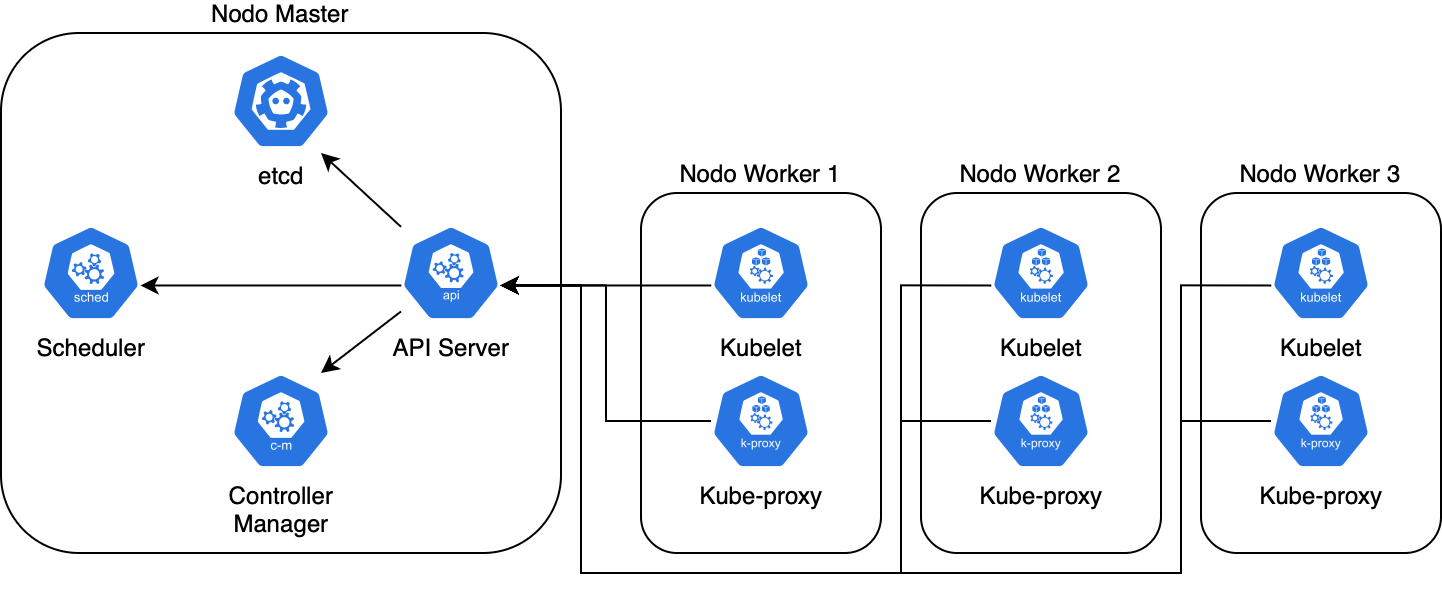
\includegraphics[width=1\linewidth]{immagini/capitolo2/kubernetes_planes.png}
    \caption{Organizzazione dei componenti Kubernetes.}
    \label{fig:kube_components}
\end{figure}

\subsection{Risorse di Kubernetes}

Kubernetes gestisce le applicazioni attraverso vari tipi di risorse, ognuna delle quali possiede un ruolo specifico:

\begin{itemize}
\item \textit{Pod}: È la più piccola e semplice unità in Kubernetes. Un Pod rappresenta una singola istanza di un microservizio e può contenere uno o più container.
\item \textit{Service}: È un'astrazione che definisce un insieme logico di Pod e la politica di accesso a essi.
\item \textit{Volume}: Fornisce storage persistente per i container in un Pod.
\item \textit{Namespace}: Permette di dividere le risorse di un cluster fisico in più cluster virtuali. Ogni namespace fornisce lo scope per i nomi delle risorse.
\item \textit{Deployment}: Permette di descrivere lo stato desiderato per i Pod o i ReplicaSet. Il Deployment Controller cambia lo stato attuale allo stato desiderato a un ritmo controllato.
\item \textit{ConfigMap} e \textit{Secret}: Forniscono meccanismi per iniettare configurazione e dati sensibili, rispettivamente, nei container.
\item \textit{Ingress}: È un'API che gestisce l'accesso esterno ai servizi in un cluster, tipicamente HTTP.
\end{itemize}
La Figura \ref{fig:kube_objects} mostra l'organizzazione delle risorse all'interno di un cluster Kubernetes.
\begin{figure}[h]
    \centering
    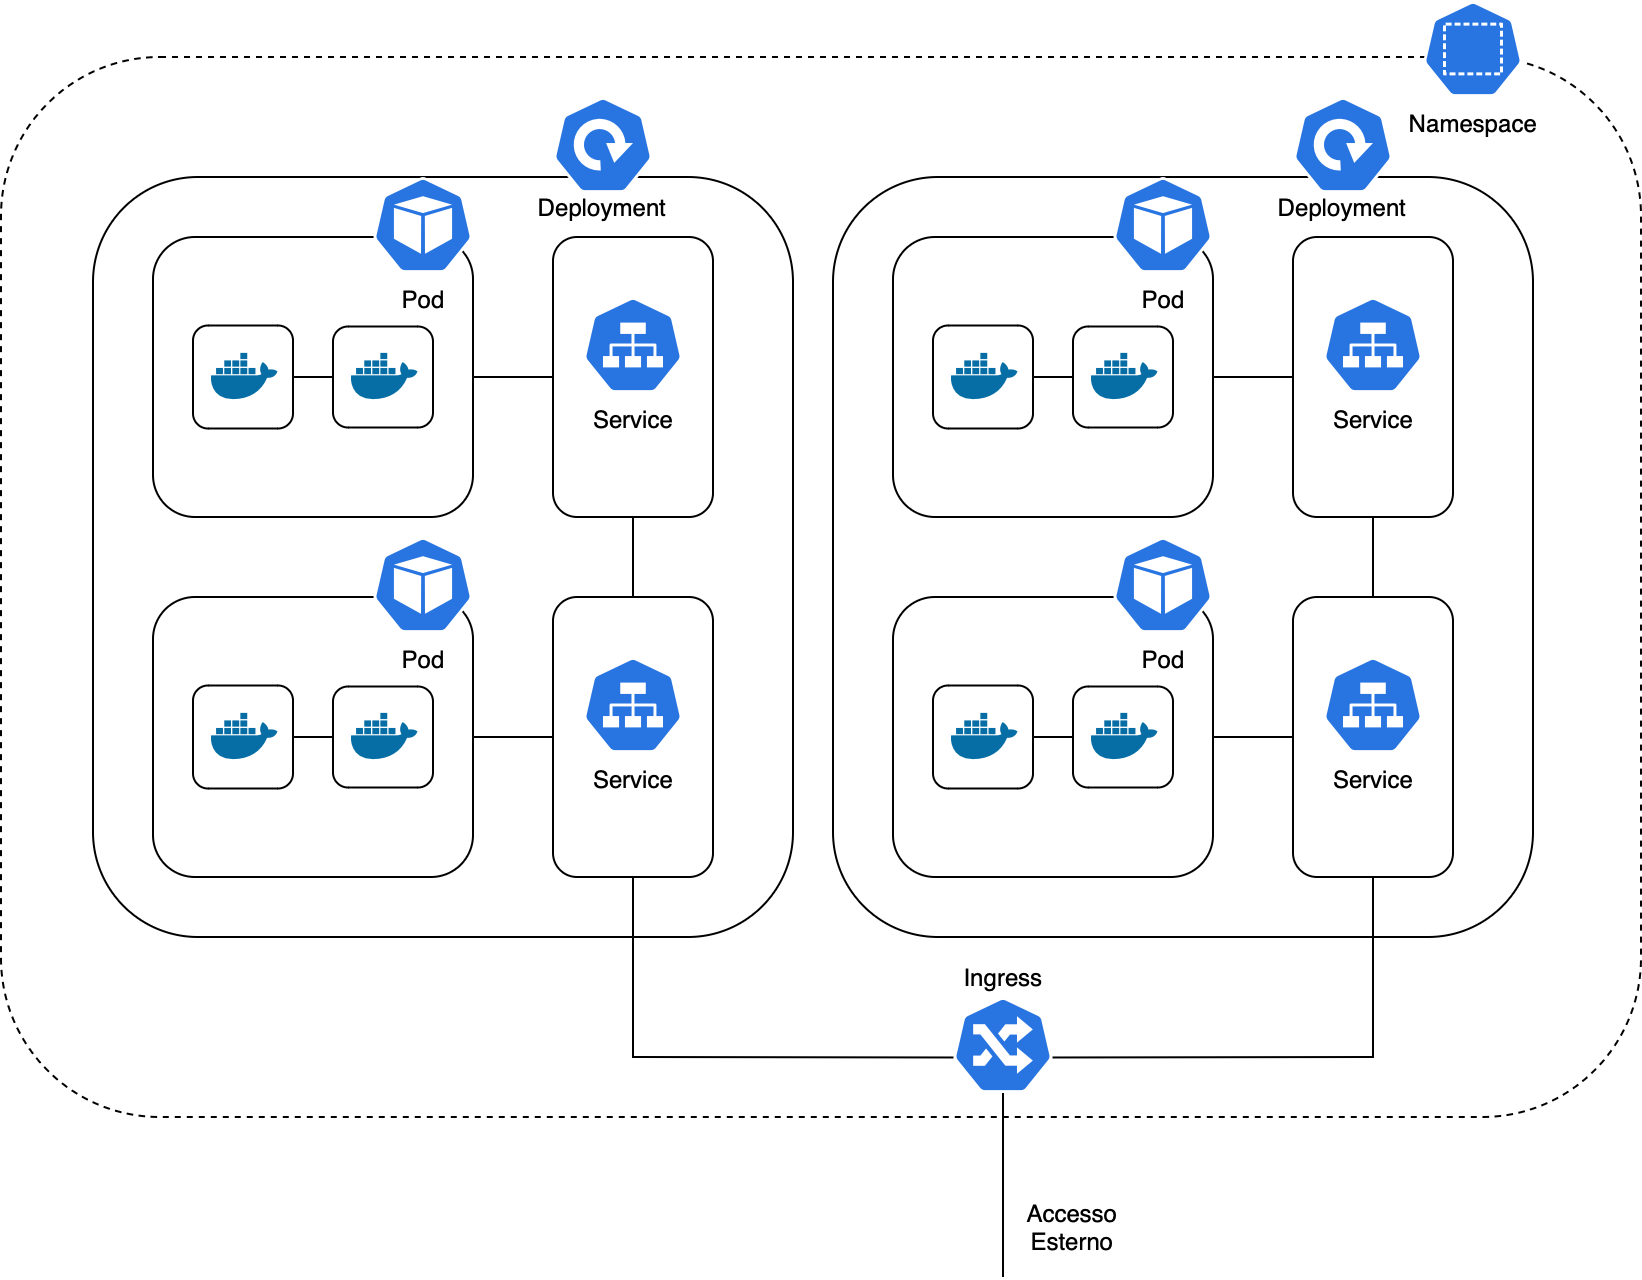
\includegraphics[width=1\linewidth]{immagini/capitolo2/kube_objects.png}
    \caption{Gerarchia e organizzazione delle risorse di Kubernetes.}
    \label{fig:kube_objects}
\end{figure}

\section{Istio}
 Per \textit{Service Mesh} si intende un livello di infrastruttura dedicato che gestisce la comunicazione tra servizi in un sistema distribuito. Questo livello può offrire una serie di funzionalità chiave, come il bilanciamento del carico, la gestione delle reti, la sicurezza e l'osservabilità dei dati, senza che siano gli sviluppatori delle applicazioni ad occuparsene in prima persona.

Tra le tecnologie nativamente integrate con Kubernetes è presente \textit{Istio}\footnote{https://istio.io}, un framework open-source per la gestione dei service mesh. \textit{Istio} fornisce strumenti avanzati per il monitoring, la tracciabilità, la sicurezza e il controllo del traffico tra i servizi. Attraverso una serie di proxy distribuiti in modo uniforme nell'ambiente, Istio riesce a intercettare e gestire il traffico di rete tra microservizi.

\subsection{Caratteristiche di Istio}
Essendo uno degli strumenti più avanzati nel suo campo, Istio offre una serie di caratteristiche distintive:

\begin{itemize}
\item \textbf{Tracciabilità e osservabilità:} Istio permette di ottenere dettagliate informazioni sul traffico, che poi possono essere utilizzati per la diagnosi di problemi nei servizi distribuiti.
\item \textbf{Controllo del traffico:} Attraverso regole e configurazioni dettagliate, Istio può determinare come il traffico viene indirizzato tra servizi, permettendo, ad esempio, un rilascio graduale o un test A/B.
\item \textbf{Sicurezza:} Istio fornisce meccanismi di autenticazione, autorizzazione e crittografia del traffico, garantendo che le comunicazioni tra servizi avvengano in modo sicuro.
\item \textbf{Bilanciamento del carico:} Oltre a semplici strategie round-robin, Istio supporta bilanciamenti più complessi basati su vari parametri e metriche.
\end{itemize}

\subsection{Componenti di Istio}

Istio è composto da due componenti principali che insieme forniscono tutte le sue funzionalità:
\begin{itemize}
    \item \textit{Istiod:} il \textit{Control Plane} della rete Service Mesh Istio
    \item \textit{Proxy Envoy:} il \textit{Data Plane} della rete Service Mesh Istio
\end{itemize}

Entrambi i componenti sono illustrati nei due paragrafi successivi.

\subsubsection{Istiod}

Istiod rappresenta il punto centrale di controllo per l'orchestrazione della Service Mesh. 
Istiod agisce da \myenquote{cervello} centrale, ricevendo configurazioni da file di tipo \texttt{yaml}, e traducendole in un formato comprensibile per il corretto funzionamento della rete. Oltre a questo, Istiod monitora continuamente l'intera mesh per assicurarsi che lo stato attuale del sistema sia conforme alle configurazioni fornite. Se ci sono discrepanze, ad esempio a causa di un guasto o di una modifica non autorizzata, Istiod interviene per correggere la situazione, garantendo così l'integrità e la sicurezza dell'intera mesh.

Nell'ambito di un'architettura di microservizi, è fondamentale garantire coerenza, sicurezza e visibilità su tutte le operazioni tra servizi. Istiod gioca un ruolo chiave in questo scenario, fornendo le seguenti funzionalità principali:

\begin{itemize}
    \item \textbf{Configurazione:} Istiod è responsabile per distribuire la configurazione a tutti i proxy Envoy presenti nella mesh. Ciò significa che ogni cambiamento o aggiornamento delle politiche, regole o configurazioni può essere propagato attraverso Istiod in maniera efficiente e sincronizzata.
    
    \item \textbf{Discovery Service:} Il componente offre un servizio di discovery per i proxy Envoy, permettendo loro di conoscere i servizi presenti all'interno della mesh e di ottenere le informazioni necessarie per il routing e il bilanciamento del carico.
    
    \item \textbf{Gestione delle Certificazioni:} Istiod gestisce anche la certificazione e la rotazione delle chiavi, assicurando che le comunicazioni tra i servizi siano crittografate e sicure. Questa funzionalità garantisce che la Service Mesh aderisca ai più alti standard di sicurezza.
    
    \item \textbf{Validazione:} Ogni volta che una nuova configurazione viene introdotta nella mesh, Istiod la valida per assicurarsi che non ci siano conflitti o errori che potrebbero compromettere il funzionamento del sistema.
    
    \item \textbf{Osservabilità:} Istiod fornisce strumenti e metriche per monitorare il comportamento e le performance della Service Mesh, permettendo agli operatori di avere una visione chiara dello stato del sistema.
\end{itemize}


\subsubsection{Proxy Envoy}

Envoy\footnote{https://www.envoyproxy.io} è un moderno proxy ad alte prestazioni progettato per applicazioni cloud-native. Sviluppato inizialmente da Lyft e ormai incluso da anni come parte integrante della rete Service Mesh Istio, funge da data plane all'interno della Service Mesh, gestendo il traffico tra i servizi e applicando le politiche e regole definite attraverso Istiod.

Le principali caratteristiche e funzionalità offerte da Envoy includono:

\begin{itemize}
    \item \textbf{Bilanciamento del Carico Dinamico:} Envoy supporta una serie di algoritmi di bilanciamento del carico e può adattarsi dinamicamente alle variazioni del sistema, come l'aggiunta o la rimozione di servizi.
    
    \item \textbf{Filtri:} Envoy offre un sistema di filtri estremamente flessibile che può essere utilizzato per manipolare e osservare il traffico in ingresso e in uscita. Ciò consente, ad esempio, di implementare funzionalità di rate limiting, logging e accesso condizionato.
    
    \item \textbf{Sicurezza:} Envoy può gestire connessioni TLS, fornendo crittografia end-to-end e garantendo che le comunicazioni tra servizi siano protette. Inoltre, in combinazione con Istiod, può effettuare autenticazioni mutue tra i servizi, rafforzando ulteriormente la sicurezza dell'intero sistema.
    
    \item \textbf{Osservabilità:} Analogamente a Istiod, anche Envoy fornisce metriche dettagliate sul traffico, latenza, errori e altro ancora, dando una visione completa del comportamento del traffico all'interno della mesh.
\end{itemize}


Il proxy Envoy è anche definito \textit{Sidecar} in quanto, quando aggiunto al sistema, Istiod modifica il deployment in modo da posizionare il proxy dentro un pod, accanto ad ogni container, ed esegue delle manipolazioni tramite la CNI (Container Networking Interface) per intercettare il traffico in ingresso ed in uscita.
\paragraph{Inserimento di Envoy in un deployment}
L'inserimento di Envoy nella rete mesh funziona tramite un meccanismo chiamato \textit{iniezione}. Per rendere possibile l'iniezione, è possibile agire su due livelli:
\begin{itemize}
\item \textbf{Livello namespace:} È possibile, sia all'atto di creazione, sia successivamente, etichettare un namespace in modo da attivare automaticamente l'iniezione di Envoy per tutti i pod che verranno creati in quel namespace. Questo può essere ottenuto applicando al namespace l'etichetta \texttt{istio-injection=enabled}, o richiedendo l'iniezione di una specifica revisione di Istio (che deve essere dotata di una specifica etichetta) tramite l'applicazione della stessa etichetta al namespace, seguendo il preciso schema \verb|istio.io/rev: <nome etichetta>|. Una volta impostate le etichette corrette, ogni pod creato nel namespace avrà automaticamente un proxy Envoy iniettato come sidecar. Questo livello di iniezione è particolarmente utile quando si desidera che tutti i servizi in un particolare namespace facciano parte della rete mesh, senza dover configurare manualmente ogni singolo pod.
\item \textbf{Livello pod:} Anche se un namespace è etichettato per l'iniezione automatica, è possibile sovrascrivere questo comportamento per singoli pod, utilizzando annotazioni specifiche nel loro deployment o nelle definizioni del pod. Questo può essere utile per escludere specifici pod dall'avere un proxy Envoy o, al contrario, per includere un pod in un namespace altrimenti escluso. L'annotazione \texttt{sidecar.istio.io/inject} può essere utilizzata per attivare (\myenquote{true}) o disattivare (\myenquote{false}) l'iniezione a livello di pod.

\end{itemize}
La Figura \ref{fig:envoy} mostra come i proxy Envoy siano dispiegati \myenquote{a fianco} dei servizi, consentendo quindi di intercettarne e gestirne il traffico.

\begin{figure}[h]
    \centering
    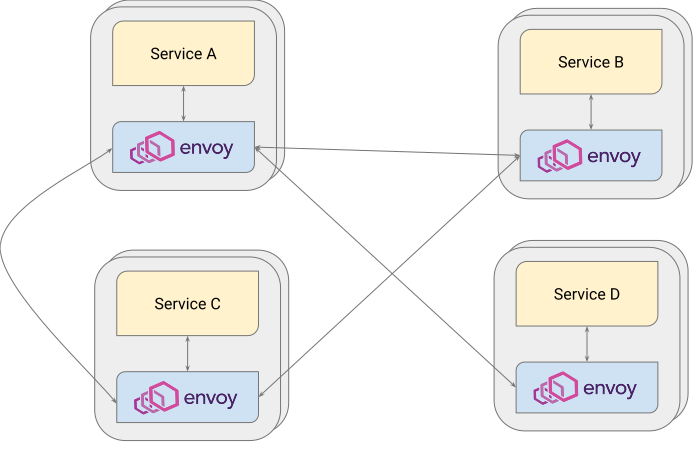
\includegraphics[width=1\linewidth]{immagini/capitolo2/envoy.png}
    \caption{Intercettazione del traffico dati da parte del proxy Envoy \cite{life_of_a_request}.}
    \label{fig:envoy}
\end{figure}


\subsection{Access Logging}

In un'era dominata dalla complessità delle applicazioni e dalla crescente necessità di trasparenza nelle operazioni digitali, monitorare e comprendere il comportamento del traffico diventa essenziale per garantire prestazioni, sicurezza e affidabilità. L'access logging, o registrazione degli accessi, è una pratica proposta come soluzione per tale problema. Questa pratica consiste nel registrare dettagliatamente ogni interazione tra un utente o un servizio e un sistema informatico. In architetture modulari e distribuite, come i microservizi, l'access logging consente di monitorare e registrare (sotto forma di log) le interazioni occorse tra i microservizi di un'applicazione ed il loro esito.

Nella rete service mesh Istio, il proxy Envoy può essere configurato per effettuare access logging, per registrare metriche riguardanti le interazioni tra le applicazioni e i servizi in un ecosistema informatico. Questi strumenti permettono di catturare, in tempo reale, informazioni dettagliate su ogni richiesta e risposta scambiata tra i servizi, facilitando così la diagnosi di problemi, l'analisi delle prestazioni e la gestione proattiva delle potenziali minacce.

All'interno di Envoy, il sistema di access logging è progettato per essere altamente configurabile. È possibile decidere quali informazioni vengono registrate, il formato in cui vengono presentate e la destinazione dei log generati. Ad esempio, è possibile catturare dettagli come l'intestazione HTTP, il corpo della richiesta, i tempi di risposta e molte altre informazioni che possono essere essenziali per la diagnosi di problemi, l'analisi delle prestazioni o la semplice revisione delle operazioni di rete.

\subsection{Integrazione con Kubernetes}

\textit{Istio} è nativamente supportato da \textit{Kubernetes}. Può infatti essere installato come un set di componenti all'interno di un cluster Kubernetes, e può automaticamente scoprire e gestire il traffico tra i pod. Questo rende particolarmente facile e potente l'uso combinato di Kubernetes e Istio per gestire applicazioni distribuite in modo scalabile e sicuro.

\section{Lo stack ELK}

Lo stack ELK, composto da ElasticSearch\footnote{https://www.elastic.co/elasticsearch/}, Logstash\footnote{https://www.elastic.co/logstash/} e Kibana\footnote{https://www.elastic.co/kibana/}, fornisce una soluzione consolidata per l'analisi e la visualizzazione dei dati, particolarmente adatta a log e dati di monitoraggio. La combinazione di ElasticSearch, Logstash e Kibana fornisce infatti un supporto flessibile per raccogliere, indicizzare e visualizzare dati in tempo reale. Lo stack ELK può essere esteso aggiungendo anche il collettore di log Filebeat, ad esempio per rendere più efficiente il processo di collezione dei log in ambienti multi-nodo.

\subsection{ElasticSearch}

ElasticSearch rappresenta uno degli strumenti più avanzati nel panorama dei motori di ricerca e analisi. Basato su Apache Lucene, framework per la ricerca full-text, ElasticSearch è stato sviluppato per soddisfare esigenze avanzate di ricerca, analisi e gestione di enormi volumi di dati in tempo reale.

Per una comprensione approfondita delle potenzialità e del funzionamento di ElasticSearch, è fondamentale introdurre alcuni concetti cardine che ne caratterizzano l'architettura:

\paragraph{Documento}
In ElasticSearch, un documento è l'unità fondamentale di informazione che può essere indicizzata. Un documento rappresenta l'unità di informazione fondamentale su cui ElasticSearch opera e può essere assimilato a un record in un database relazionale. Tuttavia, a differenza di un record tradizionale, un documento in ElasticSearch è in formato JSON e può contenere dati multivariati, quali testo, numeri, date e array. Ogni documento all'interno di un indice è identificato da un ID univoco, che permette di recuperarlo, modificarlo o eliminarlo con facilità. A differenza dei tradizionali database relazionali, dove un record deve aderire rigidamente a uno schema predefinito, in ElasticSearch ogni documento all'interno di un indice può avere una propria struttura, rendendo il sistema molto più flessibile e adattabile a vari scenari.


\paragraph{Indice}
Nel contesto di ElasticSearch, l'indice rappresenta una collezione omogenea di documenti che condividono specifiche caratteristiche o attributi. Questa definizione può essere assimilata alla struttura di una tabella in un sistema di database relazionale. Gli indici in ElasticSearch sono identificati da un nome univoco e possono essere creati, eliminati e configurati dinamicamente. Quando si crea un indice, è possibile definire una serie di impostazioni e mappature che determinano come i documenti e i loro campi sono memorizzati e indicizzati.


\paragraph{Indicizzazione}
Il processo di indicizzazione inizia quando un documento viene inviato ad ElasticSearch. Il documento, attraverso un componente denominato \myenquote{analyzer}, viene smembrato e trasformato in una serie di token. Questi analyzer sono costituiti da tokenizer e token filter. Mentre il tokenizer segmenta il testo in token basandosi su specifici delimitatori, i token filter si occupano della loro elaborazione (per esempio, conversione in minuscolo, eliminazione di parole comuni). Al termine dell'analisi, i token sono inseriti in una struttura chiamata \myenquote{inverted index}, ottimizzata per garantire ricerche veloci ed efficienti.

\paragraph{Elastic Common Schema}\label{subsubsect:ECS}
L'Elastic Common Schema (ECS) rappresenta uno standard nella definizione dei campi per i dati indicizzati su ElasticSearch. Nasce dalla necessità di avere una struttura uniforme dei dati, permettendo alle organizzazioni di semplificare la correlazione, la visualizzazione e l'analisi dei dati provenienti da fonti diverse. Grazie all'ECS, è possibile sfruttare al meglio gli strumenti offerti dalla suite Elastic, come Kibana, per creare visualizzazioni coerenti e interattive. Inoltre, l'ECS facilita l'integrazione di diverse soluzioni e fonti di dati in un ecosistema Elastic unificato, garantendo che le informazioni siano presentate in un formato comune e facilmente comprensibile.


\subsubsection{Caratteristiche distintive di ElasticSearch}

ElasticSearch è un motore di ricerca, che offre una serie di funzionalità avanzate, quali:

\begin{itemize}
\item\textbf{Scalabilità Orizzontale:} La struttura di ElasticSearch consente una facile espansione aggiungendo nodi supplementari al cluster, garantendo una gestione efficace di grandi volumi di dati e traffico.
\item\textbf{Ricerca in Tempo Reale:} L'efficienza del suo sistema di indicizzazione permette a ElasticSearch di fornire risultati di ricerca quasi in tempo reale, con latenze misurabili in millisecondi.
\item\textbf{Analisi dei Dati:} Oltre alla ricerca, ElasticSearch si distingue per le sue capacità analitiche, permettendo agli utenti di trarre intuizioni e conoscenze dai dati in tempo reale.
\item\textbf{Flessibilità:} La sua architettura è progettata per gestire sia dati strutturati che non strutturati e supporta una vasta gamma di formati, tra cui JSON e XML.
\end{itemize}


\subsection{Logstash}

Logstash è un potente strumento per la raccolta, l'elaborazione e l'invio di log ed eventi di dati ad altre piattaforme come ElasticSearch. Concepito per risolvere problemi complessi legati all'ingestione di dati, e distribuito come software open source, Logstash è stato ampiamente adottato grazie alla sua modularità e capacità di integrarsi con svariate fonti e destinazioni di dati.

\subsubsection{Funzionamento}

\paragraph{Input Plugins}
Logstash può ricevere dati da molteplici fonti, grazie ai suoi plugin di input. Che si tratti di log di sistema, flussi di eventi o dati provenienti da database, questi plugin facilitano l'ingestione di dati da svariate origini.

\paragraph{Filter Plugins}
Una volta che i dati sono acquisiti, Logstash offre una serie di plugin di filtraggio per elaborarli. Questi plugin permettono di arricchire, modificare o trasformare i dati in base alle esigenze specifiche.

\paragraph{Output Plugins}
Dopo l'elaborazione, i dati possono essere inviati a diverse destinazioni. Grazie ai plugin di output, Logstash può inviare dati a piattaforme come ElasticSearch, file, metriche, servizi cloud e molte altre soluzioni.

\paragraph{Performance e Scalabilità}

Con una progettazione orientata alla performance, Logstash può gestire volumi significativi di dati. La sua architettura supporta una scalabilità orizzontale, consentendo di distribuire l'elaborazione su più istanze e nodi.

\paragraph{Applicazioni e Casistiche d'Uso}

Logstash non si limita a essere un semplice strumento di ingestione di log. Le sue capacità di filtraggio e trasformazione rendono possibile l'uso in diversi scenari, tra cui:

\begin{enumerate}
\item \textbf{Analisi e Monitoraggio:} Integrando Logstash con ElasticSearch e Kibana, gli utenti possono creare dashboard e visualizzazioni avanzate per monitorare applicazioni, infrastrutture e servizi.
\item \textbf{Allerta e Notifiche:} Logstash può essere configurato per rilevare pattern specifici nei dati e generare allerte in tempo reale.
\item \textbf{Archiviazione Centralizzata:} Per le casistiche che necessitano di un sistema centralizzato di archiviazione dei log, Logstash offre soluzioni robuste e affidabili.
\end{enumerate}

\subsection{Kibana}

Kibana è una piattaforma di visualizzazione e dashboarding per ElasticSearch. Essa fornisce funzionalità di ricerca in tempo reale e offre la possibilità di creare visualizzazioni grafiche avanzate basate sui dati immagazzinati in ElasticSearch. Essendo l'ultimo componente dell'ELK Stack, Kibana completa il ciclo di ingestione, elaborazione e visualizzazione dei dati.

Le caratteristiche principali di Kibana sono le seguenti:

\paragraph{Interfaccia Utente Intuitiva}

Kibana è stata progettata con un'attenzione particolare all'esperienza dell'utente. La sua interfaccia grafica consente anche agli utenti meno esperti di esplorare e visualizzare i dati senza la necessità di conoscere linguaggi di query complessi.

\paragraph{Visualizzazioni Avanzate}

Dai semplici grafici a barre e linee alle mappe geospaziali, Kibana offre una vasta gamma di opzioni per visualizzare i dati. Gli utenti possono personalizzare le visualizzazioni in base alle proprie esigenze e integrarle in dashboard interattive.

\paragraph{Integrazione con ElasticSearch}

La profonda integrazione con ElasticSearch consente a Kibana di fornire funzionalità di ricerca avanzata, facilitando l'esplorazione dei dati e la creazione di visualizzazioni basate su query specifiche.


\subsection{Filebeat}

Filebeat\footnote{https://www.elastic.co/beats/filebeat} è un distributore di log che monitora i file e le directory specificate, cattura gli eventi e li invia per l'elaborazione o direttamente ad ElasticSearch. Fa parte della famiglia di prodotti Beats di Elastic e si integra nativamente con lo stack ELK, fornendo una soluzione per raccogliere dati da file di log, flussi di log di sistema o qualsiasi sorgente di dati basata su file. Di seguito, le principali caratteristiche di Filebeat:

\begin{itemize}
\item \textbf{Leggerezza:} Filebeat è progettato per essere leggero e avere un impatto minimo sulle risorse di sistema. Può essere eseguito su server, macchine virtuali e persino dispositivi IoT.
\item \textbf{Resilienza e affidabilità:} Filebeat ha la capacità di tenere traccia della posizione dei file di log letti. In caso di interruzione, può riprendere la lettura dal punto in cui si era interrotto, garantendo che non vengano persi log.
\item \textbf{Moduli integrati:} Filebeat offre moduli preconfigurati per diversi tipi di log, come Kubernetes, Apache, Nginx, e molti altri, semplificando la raccolta, la trasformazione e l'invio di dati specifici a ElasticSearch o Logstash.
\item \textbf{Integrazione flessibile:} Mentre l'integrazione diretta con ElasticSearch è comune, Filebeat può anche inviare dati a Logstash per ulteriori elaborazioni o trasformazioni prima di indicizzarli in ElasticSearch.
\end{itemize}

\subsection{Utilizzo con Kubernetes}
Se utilizzato in un cluster gestito con Kubernetes, lo stack ELK può fornire un supporto per il monitoraggio e l'analisi dei log. 
ElasticSearch può essere utilizzato per immagazzinare log da vari pods e servizi all'interno del cluster. Logstash può raccogliere questi log, eventualmente trasformarli o arricchirli, e infine inviarli a ElasticSearch per l'indicizzazione. Kibana, infine, può essere utilizzato dagli amministratori del sistema o dai team di sviluppo per analizzare questi log, identificare problemi o tendenze e prendere decisioni informate. Con l'aggiunta di Filebeat, è possibile raccogliere i log garantendo la minima occupazione delle risorse.

\section{yRCA}
yRCA\footnote{https://github.com/di-unipi-socc/yRCA} è uno strumento per l'analisi delle cause scatenanti di fallimenti osservati in applicazioni basate su microservizi. L'analisi effettuata su yRCA, nel senso che non solo vengono identificate le possibili cause di un fallimento, ma viene anche fornita una spiegazione di come tali cause possano essere risultate nel fallimento osservato.

yRCA ricerca le cause di un fallimento processando i log dei microservizi di un'applicazione, assumendo che tali microservizi emettano log per tracciare i loro fallimenti, le interazioni con gli altri servizi ed il loro esito. Sotto tale assunzione, le possibili cause di un fallimento sono identificate considerando otto scenari distinti: cinque di natura ricorsiva, associati a catene di fallimenti, e tre come casi di base, legati alle cause principali degli errori. Le cause possibili di errore di yRCA sono:

\begin{enumerate}

\item \textbf{Errore interno di un'istanza di servizio invocata:} Il fallimento loggato da un servizio A, conseguente a un'interazione non riuscita o scaduta con l'entità B, potrebbe essere risultante da un errore interno dell'entità B. In tale contesto, l'approccio si basa sull'errore interno di B per fornire una spiegazione.

\item \textbf{Interazione fallita di un’istanza di servizio invocata:} Il fallimento loggato da un servizio A potrebbe essere dovuto al fallimento dell'interazione con un servizio B, che a sua volta potrebbe essere causato da un'interazione non riuscita di B con C. Dopo aver determinato la sequenza di guasti a cascata C → B → A, l'approccio utilizza le informazioni del guasto di B per spiegare il fallimento di A.

\item \textbf{Interazione scaduta di un'istanza di servizio invocata:} Il fallimento loggato da un servizio A è stato indotto da un evento analogo in un servizio B, a seguito di un timeout nell'interazione di B con un servizio C. Una volta identificata la sequenza di timeout C → B → A, si fa riferimento al timeout di B per elaborare una spiegazione.

\item \textbf{Irraggiungibilità di un servizio invocato da un'istanza di servizio:} Il fallimento loggato da un servizio A è risultato da un timeout in un servizio B, a causa di un'interazione fallita di B. Diversamente dai precedenti casi, si considera l'ipotesi che la richiesta trasmessa da B non sia stata accettata da un servizio C, provocando quindi il fallimento per timeout. Dopo aver identificato la sequenza di guasti C → B → A, si fa riferimento al registro del timeout in B per spiegare il fallimento.

\item \textbf{Irraggiungibilità di un'istanza di servizio invocata:} Il fallimento loggato da un servizio A è nato da una richiesta non ricevuta durante l'interazione tra A e un servizio B. In questo contesto, si fa riferimento al fatto che B era irraggiungibile per fornire una spiegazione.

\item \textbf{Errore interno di un servizio:} Questa situazione interpreta un fallimento loggato da un servizio, indicando lo stesso servizio come l'origine dell'errore. La procedura ricorsiva si conclude qui.

\item \textbf{Temporanea irraggiungibilità di un servizio:} Questa situazione interpreta i fallimenti loggati da un servizio, rivelando che il servizio era temporaneamente irraggiungibile, poiché aveva registrato determinate informazioni in precedenza. La procedura ricorsiva si conclude.

\item \textbf{Servizio non avviato:} Quest'ultima situazione illustra i fallimenti loggati da un servizio, rivelando che il servizio non ha mai registrato informazioni. La procedura ricorsiva si conclude, riconoscendo che tale servizio potrebbe non essere mai stato avviato.
\end{enumerate}

\subsection{Ricostruzione delle interazioni}
Per ricostruire le interazioni, yRCA utilizza un campo chiamato \textit{request\_id}. Questo campo contiene un UUID\cite{leach_uuid_urn}, ovvero un identificativo univoco generato casualmente con lo scopo di correlare log riferenti la medesima interazione. Quando un servizio inizia un'interazione con un altro, il proxy Envoy associato al servizio chiamante genera nei propri log un UUID che viene trasmesso al proxy del servizio ricevente, e riferito a quella specifica interazione. Man mano che l'interazione si muove attraverso vari servizi o componenti, questo UUID viene trasmesso lungo la catena. Ciò permette di correlare tutti i log associati ad una singola interazione, indipendentemente da dove questi vengano generati.
\chapter{Progettazione della soluzione}\label{chap:Progettazione della soluzione}

La soluzione proposta è stata progettata con l'obiettivo di renderla indipendente sia dal tipo di deployment presentato ad essa, sia dal tipo di architettura Kubernetes. Uno degli obiettivi preposti sin dall'inizio dello sviluppo è stato infatti quello di consentirne l'utilizzo indipendentemente dal tipo di architettura Kubernetes in esecuzione sul cluster (per esempio Minikube\footnote{https://minikube.sigs.k8s.io/docs/}, kind\footnote{https://kind.sigs.k8s.io} o servizi cloud). Inoltre, l'approccio proposto è di tipo \myenquote{black-box}, quindi è progettato specificatamente per non accedere/modificare il codice dei microservizi che formano un'applicazione. Quanto presentato qui di seguito è stato quindi essenziale per raggiungere gli obiettivi descritti sopra.

\section{Separazione delle risorse in namespace dedicati}\label{sect:Spostamento delle risorse in namespace dedicati}
L'orchestrazione di applicazioni basate su microservizi con Kubernetes, richiede una gestione efficace delle risorse e una segmentazione chiara delle funzionalità. Per questo motivo, sono stati definiti tre nuovi namespace:
\begin{itemize}
\item \texttt{log-enabled:} Namespace dedicato alle risorse e ai servizi dell'applicazione di cui si vogliono ottenere, raccogliere e analizzare i log.
\item \texttt{log-istio-system:} Namespace dedicato ai componenti della rete Service Mesh di Istio.
\item \texttt{log-elk:} Namespace dedicato ai componenti dello stack ELK.
\end{itemize}



Questo approccio a namespace separati non solo mira a preservare l'integrità del dispiegamento originale, richiedendo di applicare solo modifiche minimali al file di deployment, ma fornisce uno spazio separato da tutto il resto del cluster, e dedicato unicamente per le operazioni di logging e analisi. Questa scelta si manifesta in diversi vantaggi:
\begin{itemize}
\item \textbf{Completo isolamento:} Come specificato, un namespace fornisce completo isolamento dai servizi che si trovano su altri namespace. Su Kubernetes, infatti, eventuali accessi inter-namespace possono solamente essere gestiti tramite il cosiddetto RBAC (Role-Based Access Control).
\item \textbf{Possibilità di sovrapposizione dei nomi di identificazione:} Servizi con nomi identici possono infatti coesistere sullo stesso cluster, purché essi si trovino su namespace differenti.
\item \textbf{Possibilità di sovrapposizione di numeri di porta:} Due servizi, residenti in namespace differenti, possono usare gli stessi numeri di porta per comunicare con i rispettivi destinatari, evitando quindi conflitti o interferenze.
\item \textbf{Gestione semplificata delle risorse:} Avendo namespace specifici per ogni funzione, è più facile allocare, gestire e limitare le risorse (come CPU, memoria, e storage) per ogni servizio o applicazione.
\item \textbf{Politiche di sicurezza specifiche:} Con la separazione dei namespace, è possibile definire politiche di accesso e sicurezza dedicate per ciascun ambiente.
\item \textbf{Facilità di monitoraggio:} Ogni namespace può avere metriche e dashboard dedicati, permettendo un monitoraggio più granulare e specifico.
\item \textbf{Scalabilità indipendente:} Ogni namespace può essere scalato in base alle proprie esigenze, senza influenzare gli altri namespace.
\end{itemize}

Sia per far fronte alla necessità di poter analizzare interazioni tra applicazioni che sfruttano più namespace contemporaneamente, che anche per analizzare più applicazioni allo stesso tempo, nell'implementazione è stata prevista una funzionalità che permette di specificare un suffisso per il namespace di destinazione, tipicamente riempito con il nome dell'applicazione che si vuole analizzare. Utilizzando questa opzione, il namespace di destinazione sarà del tipo \texttt{log-enabled-suffix}. Trattandosi di un'opzione facoltativa, per brevità nelle sezioni successive sarà trattato unicamente il namespace \texttt{log-enabled}, ma è importante tenere presente che ogni funzionalità che è riferita a tale namespace, è sempre applicabile anche ai namespace del tipo \texttt{log-enabled-suffix}.



\section{Configurazione della rete Istio}

\subsection{Configurazione dell'access logging}
L'interazione tra Istio e Envoy in relazione all'access logging può essere vista come una sinergia tra il controllo di livello superiore fornito da Istio e le capacità operative e dettagliate offerte da Envoy. Istio, attraverso la sua interfaccia di controllo centralizzato, permette una configurazione dell'access logging facile e uniforme per tutti i servizi che compongono la mesh. Tale configurazione viene poi tradotta e applicata in modo efficiente dal proxy Envoy, che si occupa della cattura effettiva dei log e del loro inoltro alle destinazioni designate.

Per la soluzione proposta, il formato di access logging desiderato è mostrato nel Codice \ref{lst:access_log_format}, e tale scelta è motivata dalla necessità di ricavare tutte le informazioni necessarie a yRCA \cite{tesi_spiridioni}.

\begin{lstlisting}[caption={Formato richiesto per l'ottenimento dell'access logging.}, label=lst:access_log_format, keywordstyle=\color{black}, commentstyle=\color{black},stringstyle=\color{black},numberstyle=\color{black}]
{
        "start_time": "%START_TIME%",
        "response_code": "%RESPONSE_CODE%",
        "response_flags": "%RESPONSE_FLAGS%",
        "response_code_details": "%RESPONSE_CODE_DETAILS%",
        "duration": "%DURATION%",
        "request_duration": "%REQUEST_DURATION%",
        "request_tx_duration": "%REQUEST_TX_DURATION%",
        "response_duration": "%RESPONSE_DURATION%",
        "response_tx_duration": "%RESPONSE_TX_DURATION%",
        "authority": "%REQ(:AUTHORITY)%",
        "x-request-id": "%REQ(X-REQUEST-ID)%"
      }
\end{lstlisting}
Ogni campo ha una precisa motivazione e funzionalità:
\begin{itemize}
\item \texttt{"start\_time"}: Questo campo indica l'orario di inizio di una richiesta, in termini di ora, minuto, secondo e millisecondo. Il formato utilizzato è l'ISO 8601.

\item \texttt{"response\_code"}: Rappresenta il codice HTTP inviato in risposta ad una richiesta. Questo campo può anche essere \myenquote{0}: in tal caso, significa che il servizio invocato non ha mai inviato la risposta. Solitamente, questo significa che il client si è disconnesso.

\item \texttt{"response\_flags"}: Questi flag forniscono informazioni aggiuntive sulla risposta, come ad esempio se è stata terminata prematuramente o se ci sono stati problemi nella connessione. Per la rielaborazione dei log nel formato per yRCA, vengono usati questi codici:

\begin{itemize}
\item \texttt{UF:} In aggiunta al codice di risposta 503, indica un fallimento nella connessione da parte del servizio chiamato.
\item \texttt{UC:} In aggiunta al codice di risposta 503, indica la terminazione della connessione da parte del servizio chiamato.
\item \texttt{DC:} In aggiunta al codice di risposta 504, indica la terminazione della connessione da parte del servizio chiamante.
\item \texttt{UT:} In aggiunta al codice di risposta 504, indica un evento di timeout da parte del servizio chiamato.
\end{itemize}

\item \texttt{"response\_code\_details"}: Fornisce dettagli sul codice di risposta, come ad esempio se è stato causato da un filtro specifico.

\item \texttt{"duration"}: Durata totale della richiesta del servizio chiamante, dal momento in cui viene ricevuta fino a quando viene inviata la risposta. Questo campo è espresso in millisecondi.

\item \texttt{"request\_duration"}: Tempo totale dallo \texttt{start\_time} al momento in cui l’ultimo byte viene ricevuto dal client, in millisecondi.

\item \texttt{"request\_tx\_duration"}: Tempo totale dallo \texttt{start\_time} al momento in cui l’ultimo byte viene inviato al servizio chiamato, in millisecondi.

\item \texttt{"response\_duration"}: Tempo totale dallo \texttt{start\_time} al momento in cui il primo byte viene letto dal servizio chiamato, in millisecondi.

\item \texttt{"response\_tx\_duration"}: Tempo totale dal momento in cui il primo byte viene letto dal servizio chiamato al momento in cui l’ultimo byte viene mandato al servizio chiamante.

\item \texttt{"authority"}: L'autorità di richiesta, spesso l'host HTTP. È usata per distinguere una richiesta da una risposta.

\item \texttt{"x-request-id"}: L'UUID univoco assegnato alla richiesta. Si tratta di un campo popolato dai proxy Envoy.

\end{itemize}

In casi più rari, però, ci possono essere problemi che impediscono il corretto funzionamento dell'intero pod, facendo quindi attendere il servizio chiamante un tempo indefinito in attesa di una risposta dal proxy Envoy. È necessario quindi un sistema che rilevi questo comportamento e lo interrompa, generando un messaggio di timeout. Il componente che è trattato nel paragrafo seguente è di cruciale importanza per questo scopo.


\subsection{Rilevamento dei Timeout}\label{subsect:Istio Virtual Service}
La capacità di rilevamento dei timeout è essenziale quando si tratta di analizzare fallimenti in un ambiente a microservizi. I timeout, infatti, rappresentano uno dei meccanismi chiave per identificare problemi come la latenza eccessiva, il sovraccarico di un servizio o semplicemente la mancata risposta da parte di un servizio downstream. In un sistema altamente distribuito come una mesh di servizi, il rilevamento e la gestione tempestiva dei timeout possono prevenire la propagazione di errori, migliorando la resilienza complessiva dell'applicazione.

In questo contesto, si cerca di rilevare un eventuale timeout sfruttando delle funzionalità messa a disposizione dalla rete mesh Istio.
È infatti possibile ottenere tale funzionalità tramite il concetto di \textit{VirtualService}, componente inizialmente progettato per definire e configurare le regole di routing per il traffico, ma che permette inoltre di specificare regole per la personalizzazione del tempo di timeout nelle chiamate tra microservizi differenti.

Si noti che un VirtualService non è una vera e propria entità presente in un cluster Kubernetes. Quest'ultimo è unicamente un concetto astratto che rappresenta una precisa configurazione che Istiod applica ai proxy Envoy (e, se presente nella rete, anche ad altra componentistica come l'\textit{Ingress} o \textit{Egress Gateway}). Una volta applicata la configurazione a Istiod, sarà quest'ultimo a configurare automaticamente il sidecar Envoy per il funzionamento desiderato, e a controllare periodicamente che lo stato del sistema attuale sia allineato con le configurazioni fornite.

Il Codice \ref{lst:istio_virtualservice} mostra come si presenta il file di configurazione per un VirtualService, configurato unicamente per la rilevazione di timeout.

\begin{lstlisting}[caption={Istio VirtualService per la rilevazione di timeout.}, label=lst:istio_virtualservice, keywordstyle=\color{black}, commentstyle=\color{black},stringstyle=\color{black},numberstyle=\color{black}, escapechar=|]
apiVersion: networking.istio.io/v1alpha3
kind: VirtualService
metadata:
  name: <nome del VirtualService>
  namespace: log-enabled
spec:
  hosts:
  - <nome del servizio di origine>
  http:
  - route:
    - destination:
        host: <nome del servizio di destinazione>
    timeout: 15s
\end{lstlisting}

\begin{itemize}
    \item \texttt{apiVersion:} Definisce la versione dell'API di Kubernetes. Da notare che la versione API indica l'utilizzo di una risorsa di Istio, e non nativa Kubernetes.
    \item \texttt{kind:} Specifica il tipo di risorsa, qui \myenquote{VirtualService}.
    \item \texttt{metadata - name:} Il nome del VirtualService. Nel contesto di questo progetto, tutti i VirtualService mantengono lo stesso nome del servizio a cui si riferiscono.
    \item \texttt{metadata - namespace:} Namespace, qui \myenquote{log-enabled}, in quanto si tratta di un componente che andrà dispiegato in quel namespace.
    \item \texttt{spec - hosts:} Elenca i servizi di origine per questo VirtualService. Nel contesto del progetto, ogni VirtualService viene assegnato unicamente ad uno e un solo Service Kubernetes.
    \item \texttt{spec - http - route - destination - host:} Nome del servizio di destinazione. Non essendoci particolari regole di routing, in questa sezione è specificato un solo host di destinazione, ovvero il servizio originale.
    \item \texttt{spec - http - route - timeout:} In questa sezione è configurato il timer con il quale il VirtualService deve emettere un messaggio di timeout. Di default, la soluzione prevede 15 secondi di timeout, ma lascia all'utente la possibilità di configurare questo periodo. Le informazioni sulla configurabilità di questo periodo saranno trattate nel Capitolo \ref{chap:Realizzazione della soluzione}.
\end{itemize}

\section{Configurazione dello stack ELK}

Come illustrato nel Capitolo \ref{chap:Fondamenti Teorici}, lo stack ELK, composto da ElasticSearch, Logstash e Kibana, con l'aggiunta di Filebeat per la collezione dei log, rappresenta una soluzione consolidata per la gestione, l'analisi e la visualizzazione dei log generati dalle applicazioni. Nel contesto di questo progetto, la centralità dello stack ELK non si limita alla raccolta e visualizzazione dei log, ma si estende ad un ruolo strategico nell'identificazione e nell'analisi dei fallimenti.

\subsection{Flusso di raccolta ed elaborazione dei log}
L'intero processo di raccolta, elaborazione, e memorizzazione dei log è basato sull'interazione tra i sistemi dello stack ELK, ed è stato progettato sin dall'inizio con l'idea di essere il più possibile scalabile, per far fronte anche a possibili carichi di lavoro più pesanti del previsto. Il processo avviene come segue:
\begin{enumerate}
\item Filebeat monitora continuamente il path \verb|/var/log/containers|, in tutti i nodi del cluster. Questo è il path standard dove vengono memorizzati i log dei cluster Kubernetes \cite{kubernetes_log_location}.
\item All'aggiunta di una nuova linea di log, Filebeat la raccoglie ed aggiunge ad essa metadati di Kubernetes. Questi metadati includono ad esempio il nome del pod, il nome del container, e il nome del worker node che eseguiva il pod.
\item I log vengono poi inviati all'istanza di Logstash, in esecuzione sullo stesso namespace.
\item Logstash raccoglie i log e, tramite un filtro JSON, riesce a rendere il più conforme possibile log di \verb|istio-proxy|, ed eventualmente anche log di applicazioni che emettono log in formato JSON, al formato ECS (Elastic Common Schema). I dettagli sull'utilizzo e le motivazioni di questo filtro saranno trattati al Capitolo \ref{subsect:Configurazione di Logstash}.
\item I log vengono poi inviati all'istanza di ElasticSearch.
\item ElasticSearch esegue quello che è chiamato \myenquote{\textit{dynamic mapping}}, creando automaticamente una mappa dei campi presenti nel log in base al loro tipo di dato. Questo permette di ottimizzare le query di ricerca e di analisi dati che saranno eseguite sull'istanza in un secondo momento.
\item Una volta archiviati su ElasticSearch, i log sono immediatamente disponibili per le operazioni di ricerca, visualizzazione e analisi. Questo rende particolarmente agevole e veloce l'individuazione di possibili problemi o anomalie all'interno del cluster.
\end{enumerate}
Inoltre, si prevede l'utilizzo di uno script per ottenere un dump dei log memorizzati nell'istanza ElasticSearch. Tale script deve consentire il download dei log, incluso il formato GELF (\textit{Graylog Extended Format}) atteso in input da yRCA.

\subsection{Configurazione di Filebeat}
La scelta di utilizzare Filebeat come collettore di log è motivata dal voler rendere il processo di raccolta dei log meno oneroso in termini di risorse. Infatti, nonostante Logstash possegga al suo interno capacità di collezione di log da file, esso necessita di molte più risorse, se comparato a Filebeat \cite{filebeat_resources}. Ad esempio, su un cluster multi-nodo, l'esecuzione di un'istanza di Logstash su ogni nodo (necessaria per collezionare log da tutti i pod) comporterebbe un overhead maggiore rispetto a Filebeat. Filebeat, invece, è un collettore di metriche progettato per essere a basso consumo di risorse, quindi dispiegando su ogni nodo un'istanza di Filebeat è possibile tenere attivo un numero molto minore di istanze di Logstash, dunque conservando le stesse funzionalità, ma ad un costo minore di CPU e RAM su ogni nodo.

La Figura \ref{fig:filebeat_multinode} mostra come avviene la collezione di log in  un cluster multi-nodo, e come sia necessaria una sola istanza di Logstash, nonostante la presenza di più nodi nel cluster.

\begin{figure}[h]
    \centering
    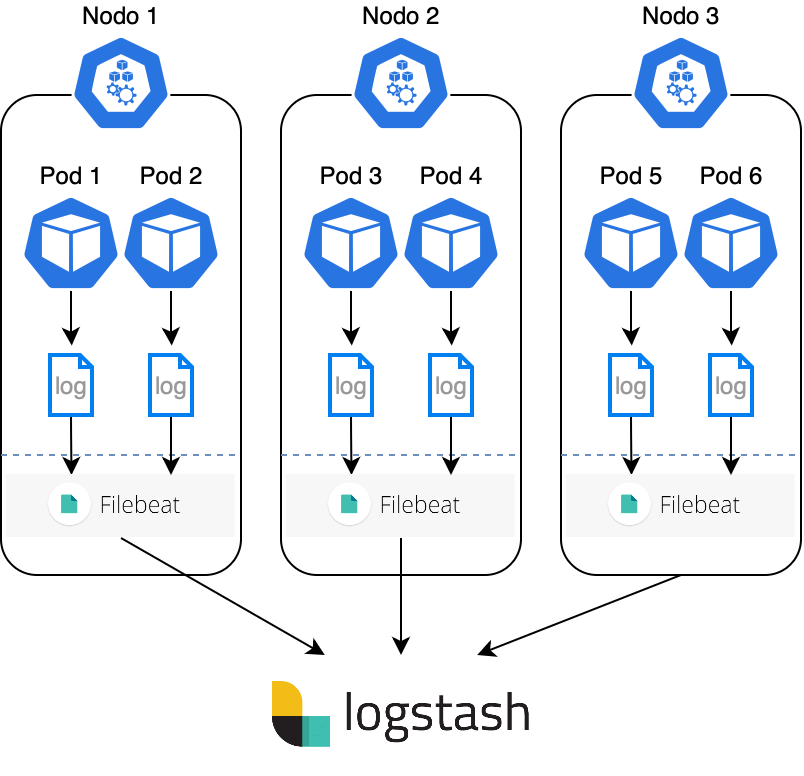
\includegraphics[width=0.75\linewidth]{immagini/capitolo3/filebeat.png}
    \caption{Funzionamento di Filebeat in un cluster multi-nodo.}
    \label{fig:filebeat_multinode}
\end{figure}

\begin{lstlisting}[caption={File di configurazione di Filebeat.},label=lst:filebeat-conf, keywordstyle=\color{black}, commentstyle=\color{black},stringstyle=\color{black},numberstyle=\color{black}]
filebeat.inputs:
- type: container
  paths:
  - /var/log/containers/*.log
processors:
  - add_kubernetes_metadata:
      host: ${NODE_NAME}
      matchers:
      - logs_path:
          logs_path: "/var/log/containers/"
  - drop_event.when.not.or:
    - contains.kubernetes.namespace: "log-enabled"
output.logstash:
  hosts: ['${LOGSTASH_HOSTS}']
\end{lstlisting}

Per gli scopi di questa tesi, Filebeat può essere configurato come mostrato in Codice \ref{lst:filebeat-conf}:
\paragraph{Filebeat.inputs}
La sezione \texttt{filebeat.inputs} specifica gli ingressi per Filebeat. Questi ingressi sono configurati per raccogliere dati dal tipo \myenquote{container}. In particolare, Filebeat è configurato per monitorare tutti i file di log nella directory \texttt{/var/log/containers/} con estensione \texttt{.log}.

\paragraph{Processors}
La sezione \texttt{processors} definisce una serie di processori che vengono applicati agli eventi raccolti da Filebeat. Il primo processore, \texttt{add\_kubernetes\_metadata}, è utilizzato per arricchire gli eventi con metadati di Kubernetes. Utilizza il nome del nodo host, specificato dalla variabile \texttt{\${NODE\_NAME}}, per ottenere questi metadati. Per determinare a quali eventi applicare questi metadati, il processore utilizza un criterio di corrispondenza basato sul percorso dei log, specificando il percorso \texttt{"/var/log/containers/"}.

Il secondo processore, \texttt{drop\_event}, ha la funzione di eliminare certi eventi basati su condizioni specificate. In questo caso, l'evento verrà scartato se non contiene il namespace di Kubernetes \texttt{log-enabled}, ovvero il namespace che conterrà il deployment target da analizzare.

\paragraph{Output.logstash}
La sezione \texttt{output.logstash} stabilisce come gli eventi raccolti da Filebeat devono essere inoltrati. In particolare, gli eventi vengono inviati a Logstash. Gli host di destinazione per Logstash sono specificati dalla variabile \texttt{\${LOGSTASH\_HOSTS}}.

\subsection{Configurazione di Logstash}\label{subsect:Configurazione di Logstash}
Logstash viene usato e configurato per elaborare opportunamente gli access log generati. In particolare, l'utilizzo principale dell'istanza di Logstash aggiunto al deployment di un'applicazione risiede nell'uniformare log che arrivano dalle varie istanze di Filebeat in modo da memorizzarli tutti nello stesso formato JSON.


Nel Codice \ref{lst:logstash-conf}, viene mostrato come configurare un'istanza di Logstash per assolvere agli scopi descritti sopra:
\begin{lstlisting}[caption={File di configurazione di Logstash.},label=lst:logstash-conf, keywordstyle=\color{black}, commentstyle=\color{black},stringstyle=\color{black},numberstyle=\color{black}]
input {
  beats {
    port => 5044
  }
}
filter {
  if [message] =~ /^{.*}$/ {
    json {
      source => "message"
      tag_on_failure => ["_jsonparsefailure"]
    }
  }
}
output {
  ElasticSearch {
    hosts => "${ElasticSearch_HOSTS}"
    index => "logstash-%{+YYYY.MM.dd}"
  }
}
\end{lstlisting}

\paragraph{Input}

Nella sezione di \texttt{input}, l'unica linea presente imposta Logstash per accettare eventi dall'istanza Filebeat sulla porta 5044.

\paragraph{Filter}

La sezione \texttt{filter} viene utilizzata per processare e trasformare gli eventi che attraversano Logstash prima che vengano inviati all'output. In questa configurazione specifica, c'è un filtro condizionale che verifica se il campo \texttt{message} di un evento contiene una stringa JSON (identificata dalla presenza di parentesi graffe all'inizio e alla fine della stringa). Se la condizione viene soddisfatta, il filtro \texttt{json} viene applicato per analizzare il campo \texttt{message} e convertirlo in un oggetto JSON strutturato. Se l'analisi fallisce, viene applicato un tag \texttt{\_jsonparsefailure} all'evento, il che può aiutare nella diagnostica e nel troubleshooting.

\paragraph{Output}

Nella sezione \texttt{output}, gli eventi processati sono inviati all'istanza ElasticSearch. Questa configurazione specifica l'endpoint di ElasticSearch utilizzando la variabile di ambiente \texttt{ElasticSearch\_HOSTS} (definita nel file di deployment di ElasticSearch). Gli eventi sono poi indicizzati in indici con un formato di nome specifico, \texttt{logstash-\%{+YYYY.MM.dd}}, che suddivide gli eventi in base alla data in cui sono stati ricevuti. Questo schema di naming consente di gestire facilmente la rotazione e la conservazione dei dati nel tempo.

\section{Architettura risultante dalla configurazione proposta}

La Figura \ref{fig:full_diagram} fornisce una visuale completa dell'architettura risultante dalla configurazione proposta, per il deployment di due servizi in un cluster Kubernetes. I due servizi sono dispiegati in due container separati, ciascuno eseguito in un pod separato. I pod sono equipaggiati con proxy Envoy, gestiti da Istio e configurati in modo da emettere gli access log come descritto nella Sezione 3.2. I log emessi dal container e dal proxy Envoy in ciascun pod sono prelevati da Filebeat e mandati a Logstash. Quest’ultimo procede alla loro conversione nel formato unificato e li spedisce ad ElasticSearch, il quale li memorizza. L’accesso ai log memorizzati può essere fatto tramite l’interfaccia offerta da Kibana, ma anche scaricando un dump dei log memorizzati direttamente da ElasticSearch.

\begin{figure}[h]
    \centering
    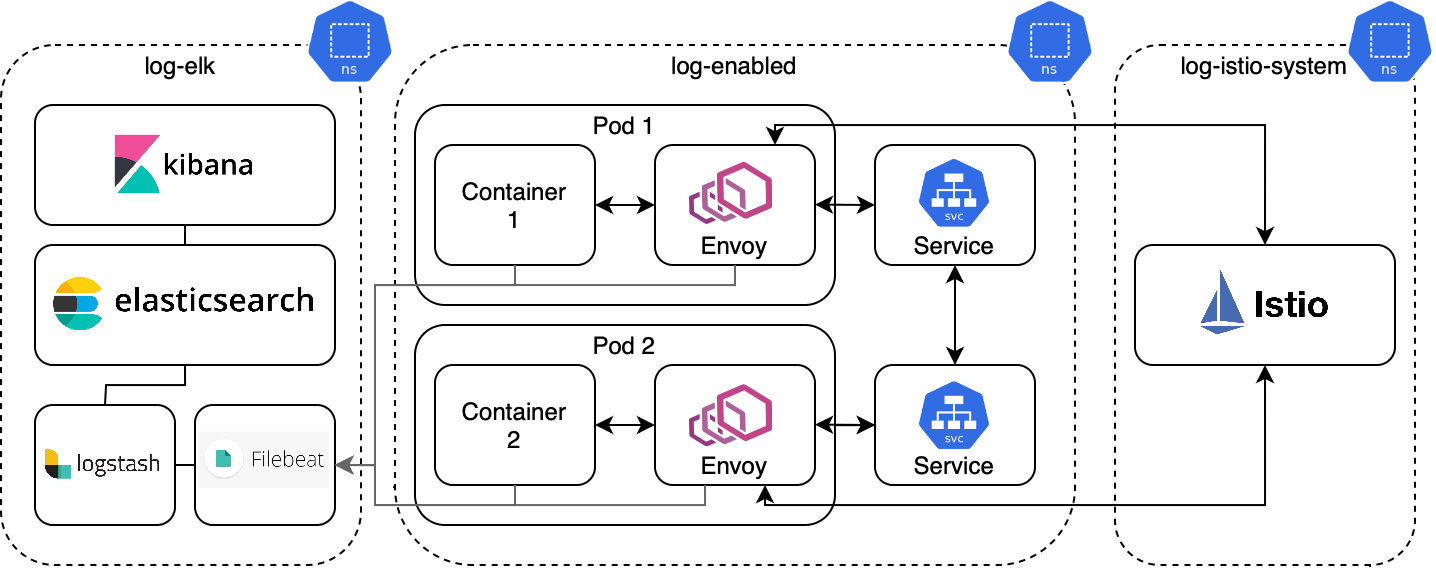
\includegraphics[width=1\linewidth]{immagini/capitolo3/full_diagram.png}
    \caption{Diagramma completo dell'architettura del sistema.}
    \label{fig:full_diagram}
\end{figure}
\chapter{Realizzazione della soluzione}\label{chap:Realizzazione della soluzione}

\section{Introduzione}\label{chap:Introduzione}
Questo capitolo introduce i file e lo strumento Python sviluppati per estendere un file di tipo manifest Kubernetes, in modo da includere i componenti che dotano il cluster delle capacità di logging richieste.
È possibile applicare tutti i componenti tramite il comando:
\begin{lstlisting}[language=bash,label=lst:kubectl-apply,]
kubectl apply -f <file.yaml>
\end{lstlisting}
E in seguito, rimuovere il tutto tramite:
\begin{lstlisting}[language=bash]
kubectl delete -f <file.yaml>
\end{lstlisting}

Non si permette, infatti, nessuna esecuzione di script o codice arbitrario, in quanto non è possibile prevedere l'architettura del cluster di destinazione: l'unica interazione che si ha sul cluster è con i comandi suddetti.

L'implementazione della soluzione proposta si divide in due fasi: la prima riguarda l'ottenimento dei file necessari per dispiegare tutti i componenti che la costituiscono. Nella seconda fase, si passa invece all'implementazione del programma che modifica automaticamente un deployment per renderlo conforme all'obiettivo della tesi.

È possibile trovare il codice completo nella repository GitHub riportata di seguito.

\verb|https://github.com/belgio99/k8s-log-enabler|.

Sono inoltre presenti tutti i dispiegamenti utilizzati per la fase di validazione, tutti i log prodotti, e metriche dettagliate per l'analisi della latenza della soluzione proposta.


\section{Ottenimento e preparazione dei file necessari}\label{sect:Ottenimento e preparazione dei componenti}

\subsection{Creazione del file manifest di Istio}\label{subsec:Creazione del file manifest di Istio}
Per l'ottenimento di un file manifest \myenquote{vergine} di Istio da poter poi inserire nella repository del progetto, è stato usato lo strumento da riga di comando \verb|istioctl|\footnote{https://istio.io/latest/docs/reference/commands/istioctl/}. Questo strumento, infatti, è dotato di una funzionalità che permette la creazione di un file predefinito, in seguito applicabile ad un cluster Kubernetes non provvisto della suddetta utility installata.

Il comando necessario per la creazione del file è riportato nel Codice \ref{lst:istioctl_manifest_generate}.
\begin{lstlisting}[caption={Comando per la creazione del file manifest di Istio.}, label=lst:istioctl_manifest_generate]
istioctl manifest generate \\
-r logrevision \\
--set profile=minimal \\
--set meshConfig.accessLogFile=/dev/stdout  \\
--set meshConfig.accessLogFormat={...}  \\
--set meshConfig.accessLogEncoding=JSON  \\
--set namespace=log-istio-system \\
--set values.global.istioNamespace=log-istio-system \\
> istio_manifest.yaml
\end{lstlisting}

Scendendo nel dettaglio, il funzionamento di ogni parte del comando è descritto nella lista sottostante:
\begin{itemize}

\item \texttt{-r logrevision}: Opzione che specifica la revisione dell'installazione di Istio. La motivazione dettagliata di questa opzione è presente al Capitolo \ref{subsubsect:Uso delle revisioni di Istio}.

\item \texttt{--set profile=minimal}: Opzione che configura Istio utilizzando un profilo minimale, che installa solo il componente principale \verb|istiod|. Questo componente, infatti, è l'unico necessario per rendere possibile la funzione di access logging.
La lista completa di tutti i profili Istio è riportata in Figura \ref{fig:istio_profiles}:
\begin{figure}[h]
    \centering
    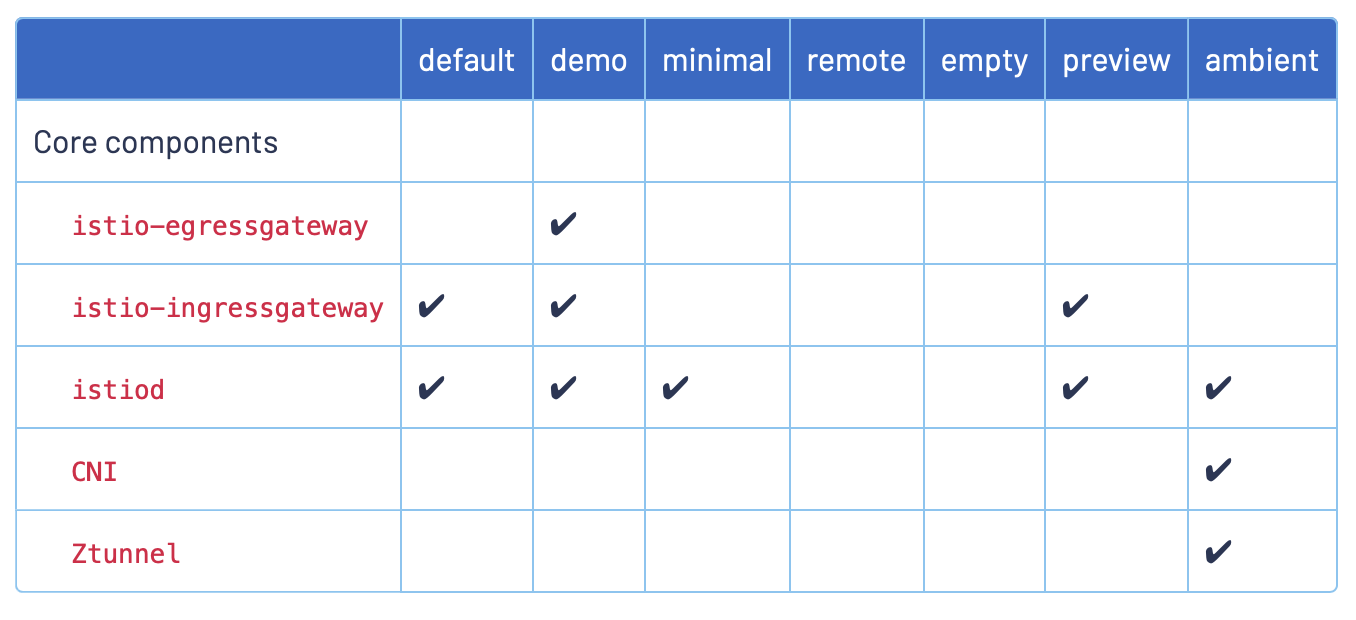
\includegraphics[width=1\linewidth]{immagini/capitolo4/istio_profiles.png}
    \caption{Tabella dei profili Istio disponibili \cite{istio_profiles}.}
    \label{fig:istio_profiles}
\end{figure}

\item \texttt{--set meshConfig.accessLogFile=/dev/stdout}: Parametro che redirige i file di log della rete mesh al flusso standard di output, in modo tale da essere poi direttamente raccolti da Filebeat senza ulteriori configurazioni.

\item \texttt{--set meshConfig.accessLogFormat=\{...\}}: Opzione che permette di definire un formato specifico per i log di accesso. Per brevità, nel comando soprastante questa parte è stata omessa, ma è disponibile nella sua interezza nel Codice \ref{lst:access_log_format}, presente al capitolo \ref{lst:access_log_format}.


\item \texttt{--set meshConfig.accessLogEncoding=JSON}: Determina il formato di codifica dei log di accesso. In questo caso, il formato è di tipo JSON, per rendere i log analizzabili da Logstash.

\item \texttt{--set namespace=log-istio-system}: Questo parametro specifica il namespace in cui Istio verrà installato. La scelta di un namespace dedicato, come \myenquote{log-istio-system}, è trattata al Capitolo \ref{sect:Spostamento delle risorse in namespace dedicati}.

\item \texttt{--set values.global.istioNamespace=log-istio-system}: Parametro che modifica un valore specifico all'interno del file di configurazione di Istio, per specificare il namespace nel quale deve cercare il suo \textit{control plane}.

\item \texttt{> istio\_manifest.yaml}: Questa parte finale del comando redirige l'output del comando precedente, ovvero il manifest generato, in un file chiamato \myenquote{istio\_manifest.yaml}, invece di stamparlo a schermo.

\end{itemize}

\subsection{Precauzioni adottate per evitare conflitti}

Nonostante il comando riportato nel paragrafo \ref{subsec:Creazione del file manifest di Istio} generi un file \verb|yaml| conforme alle specifiche di Istio per il deployment dello stesso senza \verb|istioctl|, è stato necessario prendere ulteriori precauzioni per evitare qualsiasi possibile conflitto con deployment già presente sul cluster.

Infatti, nonostante la creazione di namespace separi il più possibile le risorse, alcune di esse sono globali (dette anche \myenquote{\textit{cluster-wide}}) e possono interferire o essere interferite da risorse simili esistenti nel cluster. A causa di ciò, è necessario assicurarsi che ogni componente del file manifest di Istio sia adeguatamente configurato per evitare conflitti e rispettare le specifiche del progetto.

In particolare, sono state necessarie le seguenti modifiche:

\subsubsection{Uso delle revisioni di Istio}\label{subsubsect:Uso delle revisioni di Istio}
Negli ambienti dove può essere presente più di un control plane di Istio, è necessario un sistema di separazione ulteriore a quello provvisto dai namespace. Infatti, la separazione creata da questi ultimi non è sufficiente a garantire un isolamento completo dei control plane di Istio, visto il funzionamento inter-namespace del sistema. Per far fronte a questa necessità, gli sviluppatori di Istio mettono a disposizione il concetto di \textbf{revisione}: questa caratteristica può essere utilizzata per gli upgrade o per sperimentare con diverse configurazioni di Istio, senza influenzare il funzionamento globale. Ogni revisione di Istio viene identificata da un'etichetta unica, garantendo che le risorse siano separate e che non entrino in conflitto l'una con l'altra \textit{(Figura \ref{fig:revs})}.

\begin{figure}[h]
    \centering
    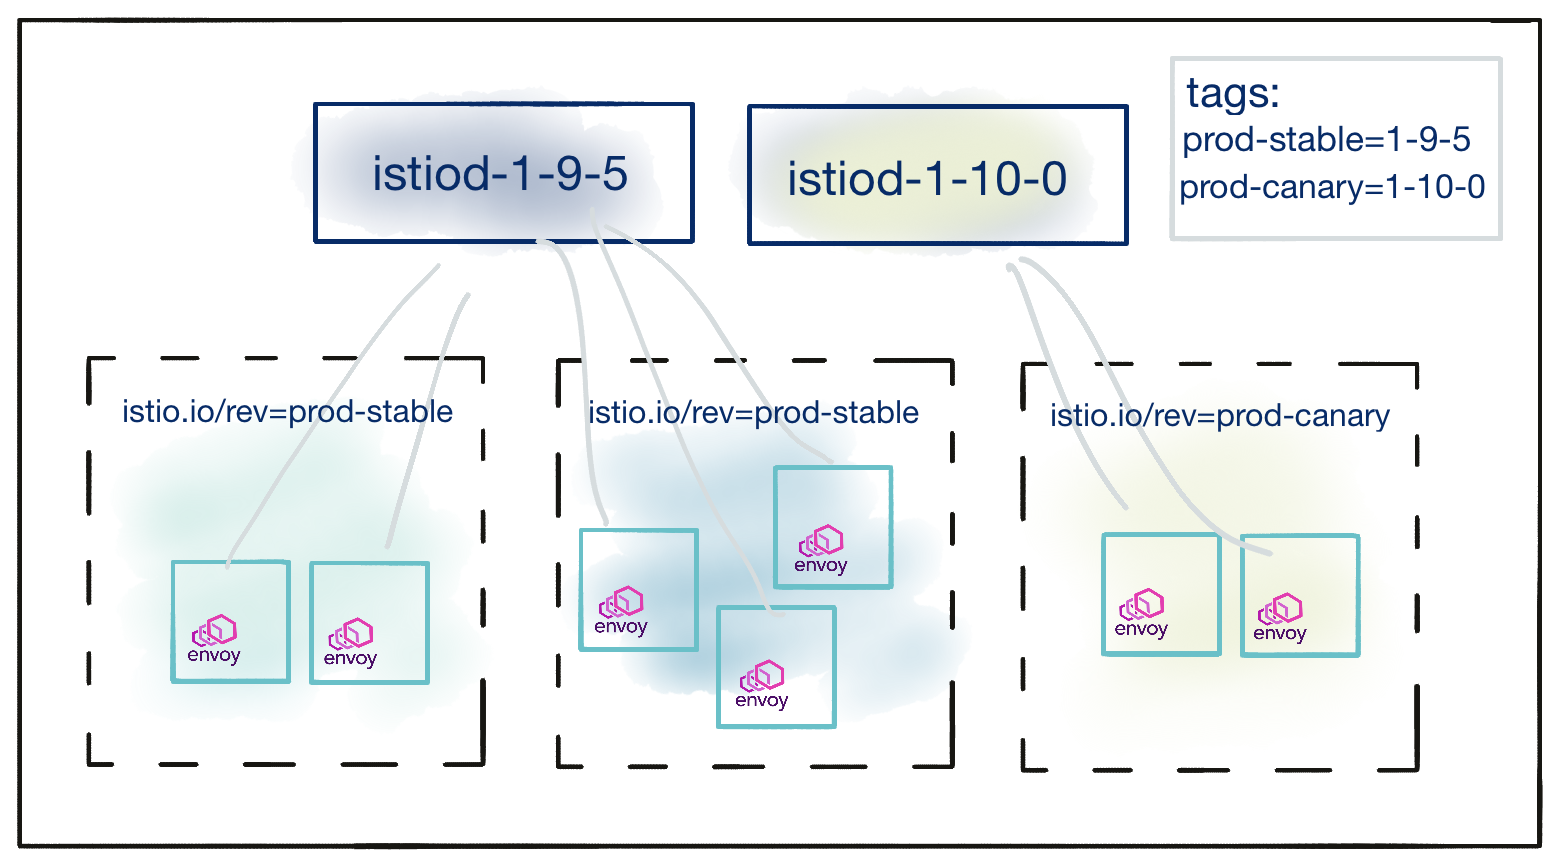
\includegraphics[width=\textwidth]{immagini/capitolo4/tags.png}
    \caption{Utilizzo tipico delle revisioni di Istio \cite{istio_revisions}.}
    \label{fig:revs}
\end{figure}



Nel contesto di questo progetto, l'utilizzo delle revisioni rende impossibile il verificarsi di una doppia iniezione del sidecar Envoy (la versione fornita nel progetto, e la versione eventualmente già presente in un cluster), in quanto l'iniezione segue queste precise regole:
\begin{itemize}
\item La revisione del control plane deve corrispondere con l'etichetta della revisione nel namespace (o nel pod) per cui si sta richiedendo l'iniezione.
\item Se nel namespace esistono più etichette di revisione, verrà utilizzata quella specificata nel pod. Se non è specificata alcuna etichetta nel pod, Istio non inietterà il sidecar.
\item Se non esiste alcuna etichetta di revisione nel namespace o nel pod, verrà utilizzato il control plane di default (se presente), ovvero il control plane che non possiede alcuna etichetta di revisione. Se quest'ultimo non è presente, l'iniezione non verrà effettuata.
\end{itemize}

Nel caso specifico, è stata utilizzata l'opzione \texttt{-r logrevision} nel comando di creazione del manifest per assegnare una revisione alla versione di Istio fornita nel progetto, come menzionato nella sezione precedente. Questa revisione consente di identificare e distinguere l'installazione di Istio dedicata alla funzione di access logging dalle altre potenziali installazioni di Istio presenti nel cluster.

Di conseguenza, è stata applicata l'etichetta \verb|istio.io/rev: logrevision| al namespace \verb|log-enabled|, per poter consentire alla versione di Istio fornita nel progetto l'iniezione del sidecar Envoy configurato per l'access logging solo su tale namespace.

\subsubsection{Separazione delle estensioni CustomResourceDefinitions}
Le \textit{CustomResourceDefinitions} (CRD) in Kubernetes sono estensioni dell'API che consentono di definire tipi di risorse personalizzate. Istio si avvale delle CRD per definire e configurare vari componenti che non rientrano nelle risorse native di Kubernetes.

Poiché le CRD sono globali all'interno di un cluster Kubernetes, esiste un rischio concreto di conflitto con altre installazioni di Istio se le definizioni fornite nel progetto interferiscono con CRD già esistenti, specialmente durante il processo di eliminazione delle risorse. Di conseguenza, si è deciso di adottare delle precauzioni nella gestione delle CRD di Istio.

Entrando più nel dettaglio, il comando spiegato alla sezione \ref{subsec:Creazione del file manifest di Istio} crea automaticamente un unico file contenente sia CRD che componenti di Istio. Dato che l'obiettivo è invece quello di poter condividere il cluster con eventuali componenti Istio già presenti, un'eventuale eliminazione delle CRD di Istio comprometterebbe il funzionamento dei componenti in esecuzione sugli altri namespace (come ad esempio il predefinito \verb|istio-system|).

Separando quindi CRD e componenti, qualora fosse già in esecuzione un'installazione di Istio in un altro namespace, è possibile saltare il passaggio di applicazione delle CRD.

\subsection{Creazione del file manifest per lo stack ELK}\label{reazione del file manifest per lo stack ELK}
Per la creazione del file manifest dello stack ELK, che è stato appositamente realizzato e configurato per questo scopo, sono stati necessari i seguenti componenti:
\begin{itemize}
\item \textbf{ServiceAccount, ClusterRole, e ClusterRoleBinding:} Componenti che forniscono a Filebeat le possibilità di interagire con le API di Kubernetes. In questo modo, è possibile arricchire i log con metadati di Kubernetes come namespace e nome del pod.

\item \textbf{Configmap:} Componenti contenenti i file di configurazione delle applicazioni Logstash e Filebeat.

\item \textbf{StatefulSet per ElasticSearch:} Componente che permette di mantenere uno stato consistente tra varie istanze di ElasticSearch. Ciò garantisce che ogni pod abbia un identificatore unico, rendendo possibile la scalabilità orizzontale del cluster in futuro.

\item \textbf{Deployment per Logstash, Kibana e Filebeat:} Per queste componenti non è necessario mantenere uno stato persistente tra le distribuzioni. Pertanto, è stato utilizzato un Deployment per gestire la loro distribuzione e scalabilità.

\item \textbf{Servizi:} I servizi per ElasticSearch, Logstash e Kibana sono necessari per permettere la comunicazione tra i componenti e l'accesso ai servizi da parte di altre applicazioni o utenti.

\item \textbf{DaemonSet per Filebeat:} Componente che assicura l'esecuzione di Filebeat su ogni nodo del cluster. Questo permette a Filebeat di catturare tutti i log da tutti i nodi.

\item \textbf{Volume e VolumeMounts:} Componenti utilizzati per fornire spazio di archiviazione persistente per ElasticSearch e per permettere a Filebeat di accedere ai log dei container.

\end{itemize}

\subsection{Creazione dei namespace dedicati}
Come riportato nel Capitolo \ref{sect:Spostamento delle risorse in namespace dedicati}, è stata progettata la creazione di tre nuovi namespace per separare le risorse e garantire un'organizzazione ottimale delle componenti nel cluster.

Per la creazione dei namespace, è stato aggiunto nella parte iniziale dei file l'apposito codice YAML, con le eventuali label già predisposte. Ad esempio, per il namespace \verb|log-enabled|, è stato sviluppato lo snippet del codice \ref{lst:log-enabled-creation}. In tale snippet, è possibile anche individuare la parte relativa all'etichettatura con la revisione di Istio fornita nel progetto:
\begin{lstlisting}[caption={Snippet della creazione del namespace log-enabled},label=lst:log-enabled-creation, escapechar=|]
apiVersion: v1
kind: Namespace
metadata:
  name: log-enabled
  labels:
    istio.io/rev: logrevision
\end{lstlisting}


\section{Script Python: introduzione e funzionalità di iniezione dei componenti}

Una volta ottenuti i file principali trattati dal capitolo \ref{sect:Ottenimento e preparazione dei componenti}, usati dallo script Python come sorgenti per la creazione del file .yaml finale, è necessario applicare delle piccole modifiche al deployment originale in modo che possa funzionare come richiesto. Nei paragrafi successivi, viene trattato il funzionamento dello script.

\subsection{Organizzazione dei file di progetto}
Il progetto Python è diviso in più file e cartelle:
\paragraph{Cartella radice}
\begin{itemize}
    \item \texttt{main.py:} File principale del progetto, contenente le funzioni di iniezione e di connessione ad ElasticSearch.
    \item \texttt{yrca.py:} File contenente le funzioni relative all'elaborazione di log per il formato richiesto da yRCA.
    \item \texttt{utils.py:} File contenente alcune funzioni di utilità, inserite in questo file per garantire una migliore organizzazione del codice.
    \item \texttt{requirements.txt:} File contenente tutti i moduli richiesti dal progetto, ed installabili tramite \textit{pip}.
\end{itemize}
\paragraph{Cartella \myenquote{manifest}}
\begin{itemize}
    \item \texttt{istio\_manifest.yaml:} File contenente il manifest \texttt{.yaml} di Istio, trattato nel Capitolo \ref{subsec:Creazione del file manifest di Istio}.
    \item \texttt{elk\_manifest.yaml:} File contenente il manifest \texttt{.yaml} dello stack ELK, trattato nel Capitolo \ref{reazione del file manifest per lo stack ELK}.
    \item \texttt{namespace\_manifest.yaml:} File contenente il file manifest \texttt{.yaml} relativo alla creazione del namespace che conterrà il deployment di cui ottenere i log.
\end{itemize}

\subsection{Moduli e librerie usate}
Per la stesura dello script, si sono usati i seguenti moduli e librerie:
\begin{itemize}
    \item \textit{Argparse:} Modulo della libreria standard di Python \cite{python_standard_library}, usato per facilitare la scrittura a riga di comando. Oltre alla possibilità di poter accedere ai parametri passati via riga di comando in modo molto intuitivo, include la possibilità di scrivere un \textit{help} in modo tale da guidare l'utente nella creazione del proprio comando.
    
    \item \textit{PyYaml:} Libreria esterna, inclusa per il supporto del linguaggio yaml, utilizzato da Kubernetes per il dispiegamento dei componenti.
    
    \item \textit{Elasticsearch:} Libreria esterna, aggiunta per comunicare con le API di ElasticSearch.
    
    \item \textit{Json:} Modulo standard Python che facilita l'elaborazione di file in formato JSON.
    
    \item \textit{Datetime:} Modulo standard Python che fornisce classi per manipolare date e orari. Offre funzioni per analizzare stringhe di date/tempo, fare aritmetica di date e formattare le date per la visualizzazione.
\end{itemize}

\subsection{Argomenti supportati dalla linea di comando}
Gli argomenti supportati dalla linea di comando sono:

\begin{itemize}

\item \texttt{-i, --inject} \textit{input\_file}: Inietta componenti di analisi del log nel file di input specificato.
    
\item \texttt{-o, --output}: Specifica un percorso di file di output personalizzato. Se non specificato, l'output del programma viene sempre stampato su \texttt{stdout}.

\item \texttt{-t, --timeout}: Specifica un timeout Envoy personalizzato. Se non specificato, il default è \myenquote{1m}.

\item \texttt{--no-header}: Permette di non aggiungere Istio e lo stack ELK al file di output finale. Opzione utile quando si vuole processare più file di deployment, dove basta che il primo file abbia i componenti suddetti, e non anche gli altri.

\item \texttt{-n namespace}: Permette di aggiungere un suffisso personalizzato al nome del namespace di destinazione, per consentire l'esecuzione di più applicazioni monitorabili contemporaneamente. Il nome finale del namespace risulterà quindi del tipo \texttt{log-enabled-suffisso}.

\item \texttt{-c, --connect} \textit{ElasticSearch\_instance}: Connette all'istanza di ElasticSearch specificata.

\item \texttt{-p, --port}: Specifica la porta di ElasticSearch. Il valore di default è 9200.

\item \texttt{--pod}: Scarica, dall'istanza di ElasticSearch, i log di un preciso pod (su un file, se utilizzato con -o). Non può essere utilizzato con il formato di output di log yRCA, in quanto quest'ultimo necessita esclusivamente dei log dei proxy Envoy.

\item \texttt{--dump-all}: Scarica, dall'istanza di ElasticSearch, i log di tutti i pod presenti nel namespace (su un file, se utilizzato con -o). Per la stessa motivazione del punto sopra, non può essere utilizzato con il formato di output di log yRCA.

\item \texttt{-f, --format}: Specifica il formato di output dei log. Le opzioni disponibili sono \texttt{yrca}, \texttt{gelf}, e \texttt{syslog}. Il valore predefinito è \texttt{yrca}.
\end{itemize}



\subsection{Processo di iniezione del file}
Il processo di modifica ed iniezione del file con tutti i componenti trattati nei paragrafi precedenti, avviene come segue:
\begin{enumerate}
    \item \textbf{Sostituzione del namespace di origine:} La prima azione che viene eseguita dallo script è quella introdotta nel Capitolo \ref{sect:Spostamento delle risorse in namespace dedicati}, ovvero la sostituzione del namespace di origine con il namespace dedicato alla raccolta e l'analisi di log \verb|log-enabled| (o, se specificato nel comando, \verb|log-enabled-suffisso|). Questo consente di ottenere il meccanismo di separazione dalle altre risorse nel cluster trattato nel Capitolo \ref{sect:Spostamento delle risorse in namespace dedicati}.


\item \textbf{Aggiunta degli Istio VirtualServices:}
Viene eseguito un parsing dedicato unicamente ai servizi presenti nel file di deployment, e per questi ultimi viene creato un Istio VirtualService, componente trattato nel capitolo \ref{subsect:Istio Virtual Service}, ed aggiunto in coda al file. Il componente sarà correttamente configurato con il timeout impostato dall'opzione \texttt{-t}.

\item \textbf{Unificazione dei file:}
Come ultimo passaggio, tutti i componenti menzionati vengono unificati in un solo file, in quest'ordine:
\begin{enumerate}
    \item Componenti di Istio
    \item Componenti dello stack ELK
    \item Dispiegamento da analizzare
    \item Istio VirtualServices
\end{enumerate}
\end{enumerate}

\section{Script Python: funzionalità di connessione all'istanza ElasticSearch}
La funzionalità di connessione all'istanza ElasticSearch è resa possibile tramite l'uso della libreria ElasticSearch di Python. Questa libreria fornisce un'interfaccia client di basso livello per interagire con un'istanza di ElasticSearch, per facilitare l'operazione di ricerca dei documenti.

Il funzionamento delle API di ElasticSearch è basato su un sistema di \textit{query}: per ottenere i dati desiderati, è necessario formare la query, ed inviarla tramite la funzione \texttt{connect}.

Per utilizzare le funzionalità di connessione a ElasticSearch, è stata creata nello script Python un'interfaccia che permette tre opzioni:
\begin{itemize}
    \item Lo scaricamento dei log relativi unicamente ai proxy Envoy (comportamento predefinito).
    \item Lo scaricamento dei log di un pod specifico (tramite l'opzione \texttt{--pod}).
    \item Lo scaricamento dei log di tutti i pod contenuti nel namespace \verb|log-enabled| (tramite l'opzione \texttt{--dump-all}).
\end{itemize}

\subsection{Utilizzo di ElasticSearch Scroll API per l'ottenimento dei dati}
Nell'utilizzo del programma Python, possono verificarsi casi in cui i log da scaricare possano superare un limite predefinito da ElasticSearch. Quest'ultimo, infatti, può fornire al massimo 10000 documenti per singola richiesta. Per far fronte alla possibilità che, in grandi deployment, possano essere prodotti più di 10000 documenti, si è optato per l'utilizzo della cosiddetta Scroll API \cite{scroll_api}. Il funzionamento è il seguente:
\begin{enumerate}
\item Inizialmente, viene eseguita una richiesta di ricerca a ElasticSearch specificando il parametro \textit{scroll}. Questo parametro indica la durata per la quale la ricerca sarà disponibile per lo scorrimento, permettendo così di ottenere più documenti in successione. In questa implementazione, il tempo di scorrimento è bloccato a 1 minuto.
\item La prima risposta, contenente la prima parte di documenti, includerà inoltre un ID di scroll. Quest'ultimo dovrà essere utilizzato nelle richieste successive per ottenere ulteriori documenti.

\item Continuando con questo meccanismo, è possibile ottenere tutti i documenti desiderati, superando il limite di 10000 documenti per singola richiesta. È fondamentale assicurarsi di proseguire con le richieste entro il periodo di tempo definito dal parametro \textit{scroll}, altrimenti la sessione si chiuderà, e sarà necessario iniziare nuovamente la richiesta.

\item Una volta ottenuti tutti i documenti necessari, è consigliabile chiudere la sessione di scroll utilizzando l'ID di scroll, per liberare le risorse utilizzate dalla richiesta sull'istanza ElasticSearch.

\end{enumerate}

\section{Script Python: funzionalità di esportazione dati}

Una volta che i dati sono stati ottenuti tramite l'ElasticSearch Scroll API, è necessario un post-processing per renderli disponibili nel formato desiderato all'avvio del programma.
I formati disponibili per l'esportazione dei dati sono tre:
\subsection{Formato yRCA}
Il formato di input per yRCA prevede 6 tipi di messaggi differenti. Questo formato richiede e necessita unicamente dei log dei proxy Envoy.
Il formato comprende sei tipi di messaggio, i quali sono descritti brevemente nella lista sottostante:
\begin{enumerate}
    \item \textbf{Invio della richiesta, lato client:} Prima dell'effettivo invio della richiesta, verrà emesso questo messaggio: \newline
    \texttt{"Sending message to [Other Service Name] (request\_id:[RequestId])"}

    \item \textbf{Ricezione di un messaggio, lato server:} Immediatamente dopo la ricezione della richiesta, verrà emesso questo messaggio: \newline
    \texttt{"Received POST request from [Other Service Name] (request\_id:[RequestId])"}

    \item \textbf{Invio della risposta, lato server:} Dopo l'elaborazione della richiesta e prima dell'invio della risposta (durante questo intervallo potrebbero verificarsi altre richieste), verrà emesso questo messaggio: \newline
    \texttt{"Answered to POST request from [Other Service Name] with code [Status Code] (request\_id:[RequestId])"}

    \item \textbf{Ricezione di una risposta OK, lato client:} Dopo aver ricevuto una risposta positiva, verrà emesso questo messaggio: \newline
    \texttt{"Receiving answer from [Other Service Name] (request\_id:[RequestId])"}

    \item \textbf{Ricezione di una risposta d'errore, lato client:} Nel caso in cui la risposta indichi un errore, verrà emesso questo messaggio: \newline
    \texttt{"Error response (code: [Response Code]) received from [Other Service Name] (request\_id:[RequestId])"}

    \item \textbf{Timeout expiration, lato client:} Se si verifica un errore dovuto a un timeout, verrà emesso questo messaggio: \newline
    \texttt{"Failing to contact [Other Service Name] (request\_id:[RequestId]). Root cause: [Root cause]"}
\end{enumerate}

Per potersi integrare con yRCA senza richiedere nessun processing esterno, questi sei tipi di output devono rispettare il formato di input richiesto da yRCA. Per fare ciò, i log vengono inseriti in un messaggio JSON contenente i seguenti campi:
\begin{itemize}
    \item \texttt{Severity:} la Severity dei log viene automaticamente applicata in base al tipo di messaggio di output. In particolare, questa è sempre impostata su INFO, tranne per quando vengono generati i messaggi di tipo 5 e 6 nella lista soprastante. In tal caso, la severity viene impostata su ERROR.
    \item \texttt{container\_name:} Il nome del pod che ha generato il messaggio.
    \item \texttt{event:} Uno dei sei tipi di messaggio descritti.
    \item \texttt{@timestamp:} La data e l'ora della generazione della linea, in formato ISO 8601.
    \item \texttt{timestamp:} La data e l'ora della generazione della linea, in formato ISO 8601, ma con separatori differenti.
    
\end{itemize}

In Figura \ref{lst:yrca-code}, è possibile vedere un messaggio di esempio che rispetta formato di output suddetto.

\begin{lstlisting}[caption={Formato di output per yRCA.},label=lst:yrca-code, escapechar=|, keywordstyle=\color{black}, commentstyle=\color{black},stringstyle=\color{black},numberstyle=\color{black}]
    {
    "severity": "ERROR", 
    "container_name": "k8s_checkoutservice", 
    "event": "Failing to contact paymentservice:50051 (request_id: [b7c3e034-e5a4-4797-af9a-2f66251ec6bc]). Root cause: ",
    "message": "2023-09-24 21:34:36.697 ERROR k8s_checkoutservice --- Failing to contact paymentservice:50051 (request_id: [b7c3e034-e5a4-4797-af9a-2f66251ec6bc]). Root cause: ",
    "timestamp": "2023-09-24 21:34:36.697",
    "@timestamp": "2023-09-24T21:34:36.697Z"
    }

\end{lstlisting}

\subsection{Formato GELF}

Il formato GELF (\textit{Graylog Extended Log Format}) \cite{gelf_format} è un formato di log progettato specificamente per il sistema di logging Graylog. È stato creato per superare le limitazioni dei formati dei log tradizionali consentendo un messaggio più strutturato e leggibile, grazie al formato JSON usato per specificare campi e valori.

GELF include campi standardizzati, ma può anche essere esteso con campi personalizzati in base alle esigenze. È riportato un esempio di un messaggio di log in formato GELF:

\begin{lstlisting}[caption={Esempio di messaggio in formato GELF.},label=lst:gelf-code, escapechar=|, keywordstyle=\color{black}, commentstyle=\color{black},stringstyle=\color{black},numberstyle=\color{black}]
{
  "version": "1.1",
  "host": "example.org",
  "short_message": "A short message",
  "full_message": "Backtrace here\n\nmore log informations",
  "timestamp": 1385053862.3072,
  "level": 1,
  "_user_defined_field": "user_defined_value"
}
\end{lstlisting}

Dove:

\begin{itemize}
  \item \texttt{version}: La versione del formato GELF.
  \item \texttt{host}: Il nome host o indirizzo IP del mittente.
  \item \texttt{short\_message}: Un breve messaggio descrittivo dell'evento. È obbligatorio e deve essere una stringa non vuota.
  \item \texttt{full\_message}: Un messaggio dettagliato o un backtrace, opzionale.
  \item \texttt{timestamp}: Il timestamp dell'evento, in secondi dal 1970-01-01T00:00:00Z.
  \item \texttt{level}: Il livello del messaggio, ad esempio 1 per \myenquote{alert} o 6 per \myenquote{info}.
  \item \texttt{\_campo\_personalizzato}: Qualsiasi campo aggiuntivo prefissato da un underscore (\_) è un campo personalizzato.
\end{itemize}

È importante notare che, mentre molti campi sono opzionali, GELF richiede almeno un \texttt{short\_message}. Se non si dispone di un valore utile, il valore \texttt{undefined} può essere utilizzato. I campi personalizzati possono invece essere utilizzati per arricchire i messaggi di log con informazioni specifiche del contesto, rendendo i dati di log più significativi. Nel progetto, infatti, sono stati aggiunti tre campi opzionali:
\begin{itemize}
    \item \texttt{\_namespace\_name}: Campo utilizzato per memorizzare il namespace del pod che ha generato la linea di log.
    \item \texttt{\_pod\_name}: Campo utilizzato per memorizzare il nome del pod che ha generato la linea di log.
    \item \texttt{\_container\_name}: Campo utilizzato per memorizzare il nome del container che ha generato la linea di log.
    
\end{itemize}


\subsection{Formato SYSLOG} SYSLOG \cite{gerhards_syslog_protocol} è un protocollo standard per l'invio di messaggi di log da dispositivi alla stazione di logging. Originariamente sviluppato negli anni '80, è diventato lo standard de facto per la registrazione di messaggi su Linux e su molte altre piattaforme. La struttura di un messaggio SYSLOG consiste in un header (che contiene informazioni come la data, l'ora e la sorgente del messaggio) seguito dal contenuto effettivo del messaggio.

Un messaggio SYSLOG si compone tipicamente delle seguenti parti:

\begin{itemize}
  \item \texttt{PRI}: Un numero che rappresenta la combinazione di facility e livello del messaggio. È una cifra che determina la priorità del messaggio.
  \item \texttt{HEADER}: Contiene due campi - il TIMESTAMP e il HOSTNAME del dispositivo o dell'applicazione che invia il messaggio.
  \item \texttt{MSG}: Il corpo del messaggio, che dettaglia l'evento o la situazione segnalata.
\end{itemize}

Un esempio di messaggio SYSLOG potrebbe apparire così:

\begin{lstlisting}
<34>Oct 11 22:14:15 mymachine myapp: An example message here
\end{lstlisting}

Dove:

\begin{itemize}
  \item \texttt{$<$34$>$}: Indica la PRI. È una combinazione di facility (come \myenquote{auth}, \myenquote{mail}, \myenquote{kern}, etc.) e livello (come \myenquote{emerg}, \myenquote{alert}, \myenquote{crit}, etc.). Nello script Python, questo valore è fisso a 134.
  \item \texttt{Oct 11 22:14:15}: È il TIMESTAMP, che indica quando il messaggio è stato generato.
  \item \texttt{mymachine}: Rappresenta il nome HOSTNAME del dispositivo o dell'applicazione che ha generato il messaggio.
  \item \texttt{myapp}: È il nome dell'applicazione o del processo che ha generato il messaggio.
  \item \texttt{An example message here}: È il corpo effettivo del messaggio o MSG.
\end{itemize}

\chapter{Validazione della soluzione}\label{chap:Validazione della soluzione}
Per procedere alla validazione della soluzione proposta, è stato preparato un ambiente Kubernetes in esecuzione su Minikube, che a sua volta è in esecuzione su un container Docker\footnote{https://www.docker.com}. Sebbene questo ambiente sia notoriamente più piccolo rispetto ai dispiegamenti tipici su microservizi, rimane un valido strumento per il testing della soluzione proposta, trattandosi a tutti gli effetti di un ambiente Kubernetes.

Tutti i log delle validazioni della soluzione sono disponibili nella repository del progetto, trattata al Capitolo \ref{chap:Realizzazione della soluzione}. In particolare, nella cartella \textit{output\_logs}, è presente una cartella per ogni test della soluzione proposta. La struttura dei file segue lo schema descritto di seguito:
\begin{itemize}
    \item \textit{all.log}: contiene i log di tutte le interazioni scambiate tra i microservizi.
    \item \textit{event.log}: contiene l'evento di interesse che si vuole ispezionare tramite yRCA.
\end{itemize}
\section{Iniezione di un fallimento nell'applicazione Bookinfo} \label{sect:Iniezione di un fallimento nell'applicazione Bookinfo}
\subsection{Introduzione a Bookinfo}
Istio, come la maggior parte delle piattaforme moderne, fornisce un'applicazione di esempio per aiutare gli sviluppatori a familiarizzare con le sue funzionalità. L'applicazione di esempio offerta da Istio è chiamata \myenquote{Bookinfo}\footnote{https://istio.io/latest/docs/examples/bookinfo/}. Questo capitolo fornisce una panoramica dell'applicazione Bookinfo, e come è stata usata a scopi di test per testare il funzionamento della soluzione.

Bookinfo è un'applicazione a microservizi che mostra informazioni sui libri in una sorta di negozio online. Composta da molteplici componenti, ognuno di essi si trova in un deployment separato:
\begin{itemize}
    \item \textit{Productpage:} Microservizio contenente un server Web che rende possibile la visualizzazione di una semplice pagina Web. Internamente, è anche responsabile di chiamare i servizi interni .
    \item \textit{Details:} Microservizio contenente le informazioni dettagliate dei libri.
    \item \textit{Reviews:} Microservizio utilizzato per mostrare le recensioni degli utenti. È presente in tre versioni:
    \begin{itemize}
        \item \textit{v1:} Versione che non mostra recensioni degli utenti.
        \item \textit{v2:} Versione che mostra recensioni degli utenti, con stelle nere.
        \item \textit{v3:} Versione che mostra recensioni degli utenti, con stelle rosse.
    \end{itemize}
    \item \textit{Ratings:} Microservizio chiamato dalla versione v2 e v3 di \textit{Reviews}, e produce una valutazione per un libro.
\end{itemize}

La Figura \ref{fig:with_istio} mostra il suddetto ambiente.

\begin{figure}[h]
    \centering
    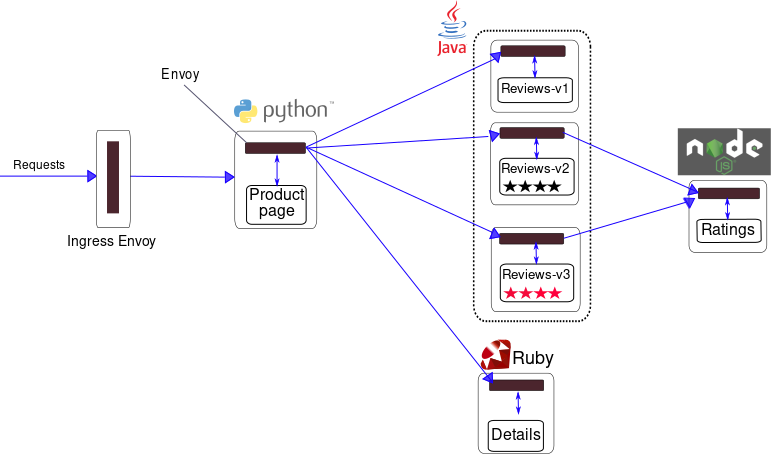
\includegraphics[width=\textwidth]{immagini/capitolo5/withistio.png}
    \caption{Schema fornito da Istio per Bookinfo \cite{istio_bookinfo}.}
    \label{fig:with_istio}
\end{figure}

Il microservizio su cui si vuole generare un fallimento per questa dimostrazione è \texttt{Ratings}, in quanto trattasi di un servizio cruciale e non ridondante.


Il metodo che sarà usato per interrompere il traffico tra \texttt{Reviews} e \texttt{Ratings} sarà quello di simulare un blocco interno al container \texttt{Ratings}, come in Figura \ref{fig:with_istio_broken}.

\begin{figure}[h]
    \centering
    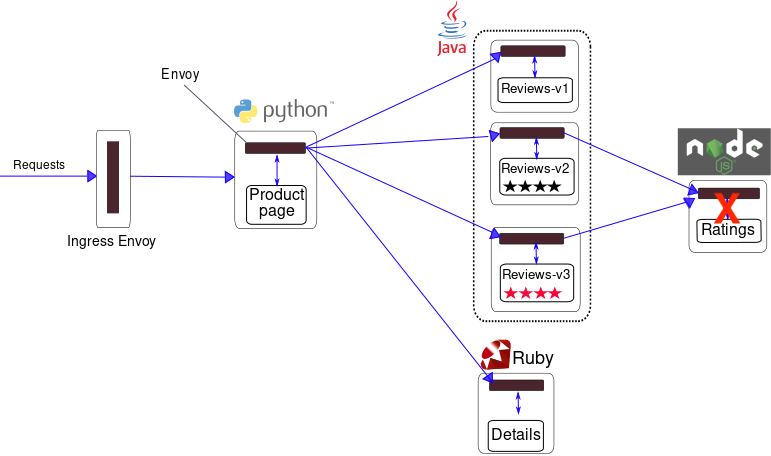
\includegraphics[width=\textwidth]{immagini/capitolo5/withistio_broken.png}
    \caption{Punto di simulazione del fallimento.}
    \label{fig:with_istio_broken}
\end{figure}


Per fare ciò, saranno usate delle funzionalità di Docker e Minikube che consentono di interrompere l'elaborazione di un container senza spegnerlo completamente. La differenza, infatti, sta nel modo in cui viene gestito questo fallimento da Kubernetes: simulando un crash del container il processo non sarebbe dimostrabile, perché Kubernetes tenta sempre di riavviare il pod o container interrotto.
\subsection{Iniezione del fallimento}\label{Iniezione del fallimento}
Per prima cosa, viene eseguito il tool Python che trasforma il deployment originale di Bookinfo in un deployment con le funzionalità di logging descritte nei capitoli precedenti. Dopo di esso, si applicano al cluster le CRD, e il deployment modificato al cluster, tramite l'esecuzione dei comandi descritti nel Codice \ref{lst:code_run_script}:

\begin{lstlisting}[caption={Comandi per l'applicazione dei CRD e del deployment modificato.}, label=lst:code_run_script, language=bash]
python main.py -i <file_input> -o <file_output>
kubectl apply -f crds.yaml
kubectl apply -f <file_output.yaml>
\end{lstlisting}
\begin{figure}[H]
    \centering
    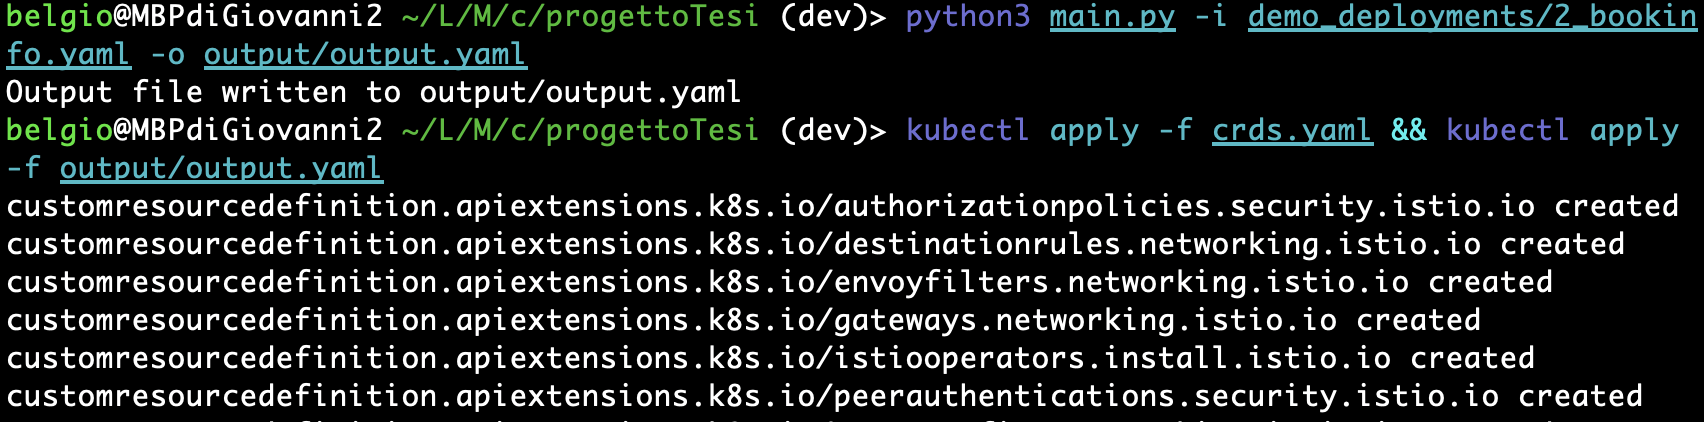
\includegraphics[width=\textwidth]{immagini/capitolo5/run_script.png}
    \caption{Esecuzione dello script Python e applicazione delle risorse al cluster.}
    \label{fig:run_script}
\end{figure}

Dopo l'esecuzione, è possibile vedere che tutte le risorse sono state dispiegate correttamente e nei namespace corretti, tramite l'esecuzione dei comandi presenti nel Codice \ref{lst:code_get_pod}, e di cui è possibile vedere l'esecuzione in Figura \ref{fig:kubectl_get_pod}.
\begin{lstlisting}[caption={Comandi per l'applicazione dei CRD e del deployment modificato.},label=lst:code_get_pod,language=bash]
kubectl get pod -n log-enabled-bookinfo
kubectl get pod -n log-istio-system
kubectl get pod -n log-elk
\end{lstlisting}
\begin{figure}[h]
    \centering
    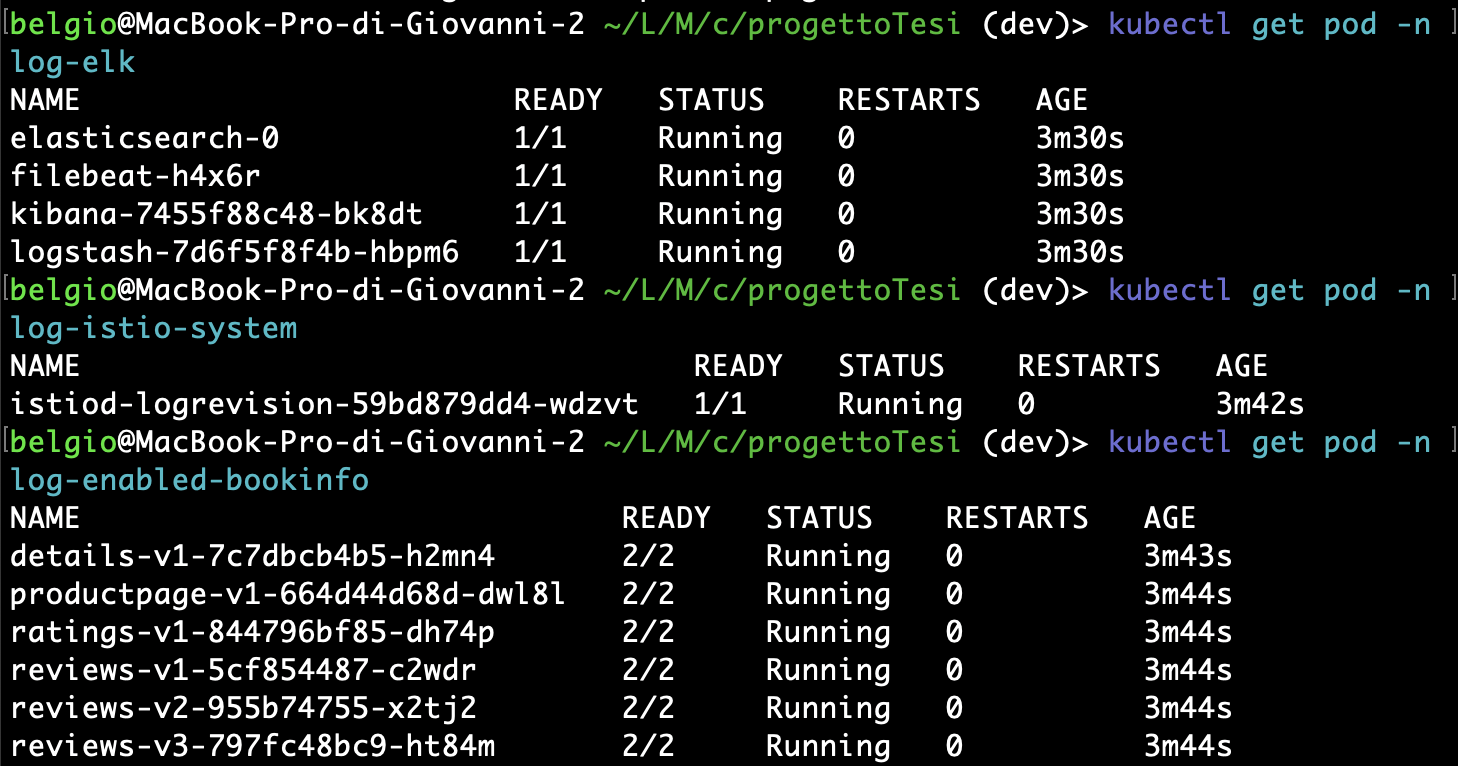
\includegraphics[width=\textwidth]{immagini/capitolo5/kubectl_get_pod.png}
    \caption{Controllo del corretto deploy delle risorse.}
    \label{fig:kubectl_get_pod}
\end{figure}

Tramite Minikube, è possibile esporre dei servizi presenti l'ambiente Kubernetes al sistema host. In particolare, il servizio interessato in questo caso è il servizio \texttt{productpage}, che consente di verificare il corretto funzionamento dello stack di servizi. Ciò è possibile tramite il comando \ref{lst:code_minikube_productpage}:
\begin{lstlisting}[caption={Esposizione del servizio \texttt{productpage} al sistema host.}, label=lst:code_minikube_productpage, language=bash]
minikube service productpage --url -n log-enabled-bookinfo
\end{lstlisting}
Come si osserva in Figura \ref{fig:working}, sia le \texttt{Reviews} che i \texttt{Ratings} vengono serviti correttamente a \texttt{Productpage}.

\begin{figure}[h]
    \centering
    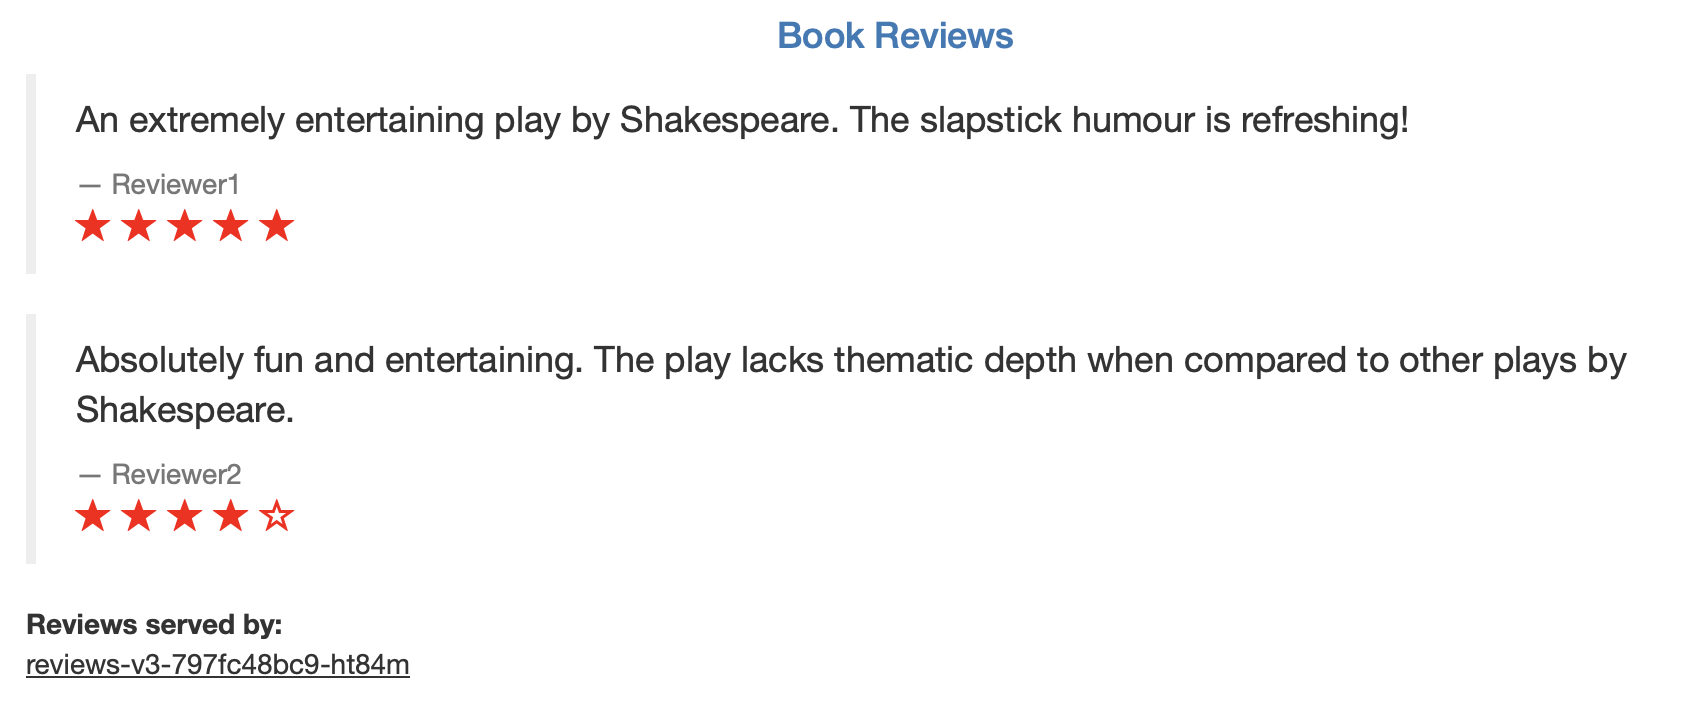
\includegraphics[width=\textwidth]{immagini/capitolo5/working.png}
    \caption{Controllo del funzionamento di \texttt{Productpage}.}
    \label{fig:working}
\end{figure}


Kubectl non mette a disposizione un comando per interrompere l'esecuzione di un fallimento, ma dato che l'ambiente di test è Minikube in esecuzione su Docker, è possibile configurare la shell locale per utilizzare il demone Docker che si trova all'interno di Minikube. Per eseguire ciò, è necessario eseguire il comando \ref{lst:shell_minikube}:

\begin{lstlisting}[caption={Passaggio al demone Docker in Minikube.}, label=lst:shell_minikube, language=bash]
eval $(minikube docker-env)
\end{lstlisting}

Utilizzando il demone Docker all'interno di Minikube, è possibile mettere in pausa l'esecuzione del container, simulando quindi un fallimento interno. Per fare ciò, è necessario eseguire il comando presente nel Codice \ref{lst:grep_ratings}: 
\begin{lstlisting}[caption={Ottenimento del container relativo ai Ratings.}, label=lst:grep_ratings, language=bash]
docker ps | grep k8s\_ratings
\end{lstlisting}

Tramite il comando del Codice \ref{lst:grep_ratings}, è possibile scoprire qual è l'ID del container di \verb|Ratings|, per poi metterlo in pausa. Nell'esempio della Figura \ref{fig:pause}, l'ID associato al container è \texttt{aa42b22e1568}.

A questo punto, è possibile interrompere temporaneamente l'esecuzione di \verb|Ratings|, tramite il comando riportato nel Codice \ref{lst:docker_pause}: 
\begin{lstlisting}[caption={Pausa del container.}, label=lst:docker_pause, language=bash]
docker pause <id_container>
\end{lstlisting}

\begin{figure}[h]
    \centering
    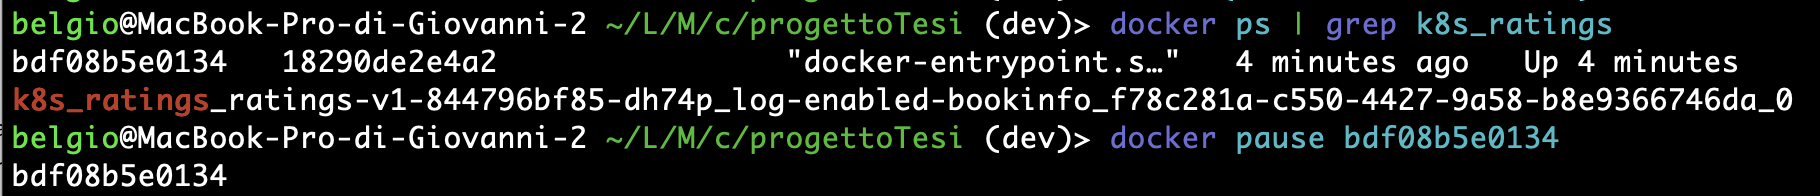
\includegraphics[width=\textwidth]{immagini/capitolo5/pause_cont.png}
    \caption{Container sospeso correttamente.}
    \label{fig:pause}
\end{figure}


Con il container in pausa, il proxy Envoy genererà una stringa di errore, che sarà poi elaborata dallo script Python per produrre l'errore in uno dei formati richiesti. È poi possibile scaricare i log richiesti dall'istanza ElasticSearch eseguendo il comando:
\begin{lstlisting}[caption={Comando per lo scaricamento dei log da ElasticSearch.}, label=lst:log_download, language=bash]
python main.py -c localhost -p <porta> -o <file di output> -n bookinfo
\end{lstlisting}

In Figura \ref{fig:cat_log}, si possono visualizzare parte dei log scaricati in questo test. Visto il lungo messaggio JSON prodotto, in figura viene evidenziata solo la parte \textit{event}:

\begin{figure}[h]
    \centering
    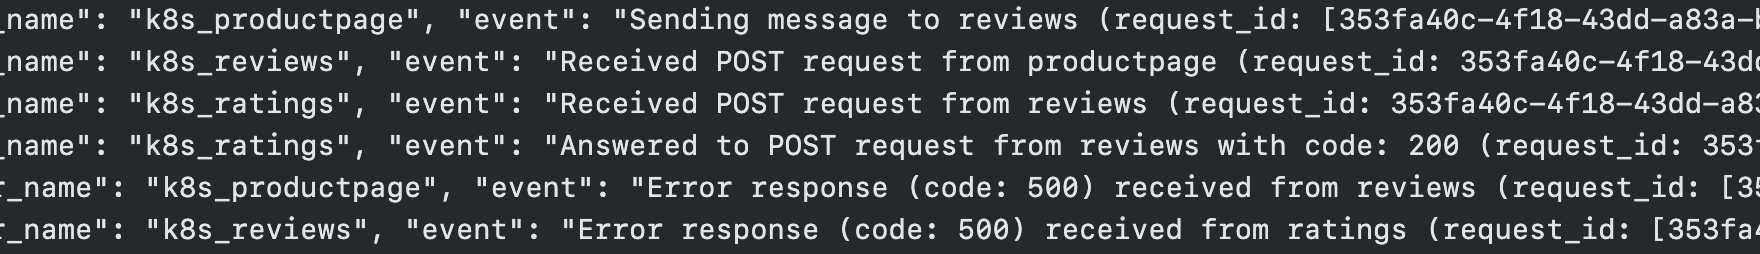
\includegraphics[width=\textwidth]{immagini/capitolo5/cat_log.png}
    \caption{Visualizzazione dei log.}
    \label{fig:cat_log}
\end{figure}

Per provare poi il corretto funzionamento del sistema, è possibile eseguire yRCA per individuare quale sia stata la causa o il motivo del fallimento: infatti, in questo caso, interrogando yRCA sul perché ci sia stato un fallimento, viene correttamente identificato da yRCA che si è trattato del container \texttt{Ratings}, non più operativo.
\begin{figure}[h]
    \centering
    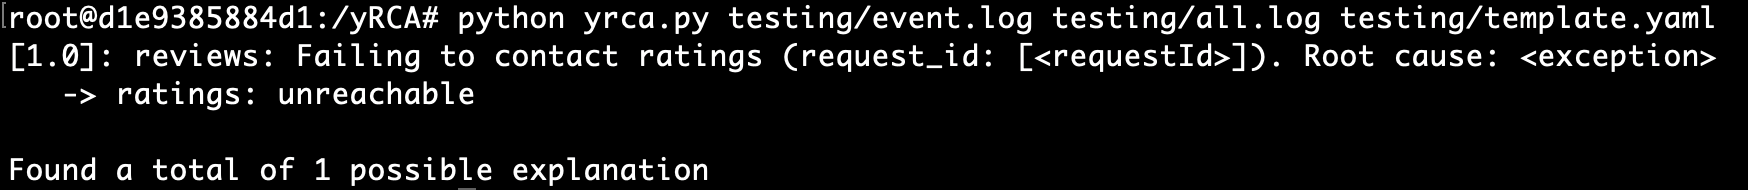
\includegraphics[width=\textwidth]{immagini/capitolo5/bookinfo_yrca.png}
    \caption{Esecuzione di yRCA per spiegare il motivo del fallimento.}
    \label{fig:yrca-error}
\end{figure}


\section{Simulazione di un fallimento con l'applicazione Chaos Echo}
\subsection{Introduzione a Chaos Echo}
Chaos Echo\footnote{https://github.com/di-unipi-socc/chaos-echo} è un'applicazione progettata per testare la resilienza ai fallimenti di un'applicazione a microservizi. Il suo funzionamento è basato sulla ricezione di richieste da parte di un'applicazione esterna, e sulla successiva risposta in maniera aleatoria: o fornendo una risposta entro un certo intervallo di tempo, o inducendo un timeout, simulando così una potenziale interruzione del servizio.

Chaos Echo permette la configurazione dei parametri interni tramite le seguenti variabili d'ambiente:
\begin{itemize}
    \item \texttt{DEPENDS\_ON}: Parametro che indica dei nomi di host che il servizio può a sua volta contattare.
    \item \texttt{TIMEOUT}: Parametro che indica il tempo di timeout, in millisecondi, con il quale si deve attendere una risposta da un servizio contattato.
    \item \texttt{P\_INVOKE}: Parametro con range da 0 a 100, con il quale si indica la probabilità in percentuale che il suddetto servizio chiami a sua volta uno dei servizi specificati nel campo \texttt{DEPENDS\_ON}.
    \item \texttt{P\_FAIL}: Parametro con range da 0 a 100, con il quale si indica la probabilità in percentuale che il servizio non risponda a richieste provenienti da altri servizi o dall'esterno.
    \item \texttt{P\_CRASH}: Parametro con range da 0 a 100, con il quale si indica la probabilità in percentuale che il servizio termini al momento di ricezione della richiesta.
\end{itemize}


In questa seconda casistica di fallimento, l'obiettivo è ancora quello di simulare un fallimento interno, ma differentemente da quanto accaduto nella prima casistica di testing, dove un blocco completo del container impediva sia la ricezione che la trasmissione di richieste e risposte, questa seconda casistica si concentra sullo sviluppare un messaggio di timeout, dove la richiesta viene ricevuta correttamente dal container, ma non viene mai elaborata una risposta, generando un timeout.

\subsection{Iniezione del fallimento}

In questa implementazione, vengono dispiegate tre istanze di Chaos Echo, ognuna con parametri di configurazione differenti:
\begin{itemize}
    \item \textit{Frontend}: \texttt{P\_INVOKE} = 100\%, \texttt{P\_FAIL} = 50\%, \texttt{P\_CRASH} = 0\%, 
    \item \textit{Middle}: \texttt{P\_INVOKE} = 100\%, \texttt{P\_FAIL} = 90\%, \texttt{P\_CRASH} = 0\%, 
    \item \textit{Backend}: \texttt{P\_INVOKE} = 0\%, \texttt{P\_FAIL} = 90\%, \texttt{P\_CRASH} = 70\%, 
\end{itemize}

Quando una chiamata HTTP parte da \textit{curl} e arriva a \textit{frontend}, quest'ultimo la redirige verso \textit{middle}, con le probabilità specificate sopra. Una volta arrivata a \textit{middle}, viene poi indirizzata verso \textit{backend}, che decide se fallire esso stesso, oppure inviare un messaggio di errore.

Per generare le chiamate, è stato creato un file di deployment Kubernetes che unisce le istanze di Chaos Echo con un container che esegue l'immagine \texttt{radial/busyboxplus:curl}\footnote{https://hub.docker.com/r/radial/busyboxplus}. L'unico scopo di quest'ultimo container è eseguire il comando \textit{curl}, e di attendere un tempo predefinito tra una chiamata e l'altra, in modo da simulare le chiamate provenienti da un eventuale servizio esterno.
Il comando utilizzato per tale scopo è:
\begin{lstlisting}
    curl -X POST -H 'Content-Type: application/json' -H 'Cache-Control: no-cache' -i http://$A/echo --data '{ "content": "FRONTEND REQUEST", "hash": "1" }' --silent & 
\end{lstlisting}
Per l'iniezione del fallimento i passi necessari per il dispiegamento del deployment sono identici a quanto descritto per Bookinfo, ma utilizzando Chaos Echo come deployment target. Come richiesto dalla specifica del test, il container con curl inizia a inviare richieste alle istanze di Chaos Echo, e provoca fallimenti di tipo timeout quando la richiesta non viene risposta entro un tempo limite. In questo test, il tempo massimo consentito per l'invio di una risposta prima della generazione dell'errore di timeout è stato fissato ad 1 secondo. In Figura \ref{fig:chaosecho-logs}, sono riportati i messaggi di errore estratti dai log.

\begin{figure}[h]
    \centering
    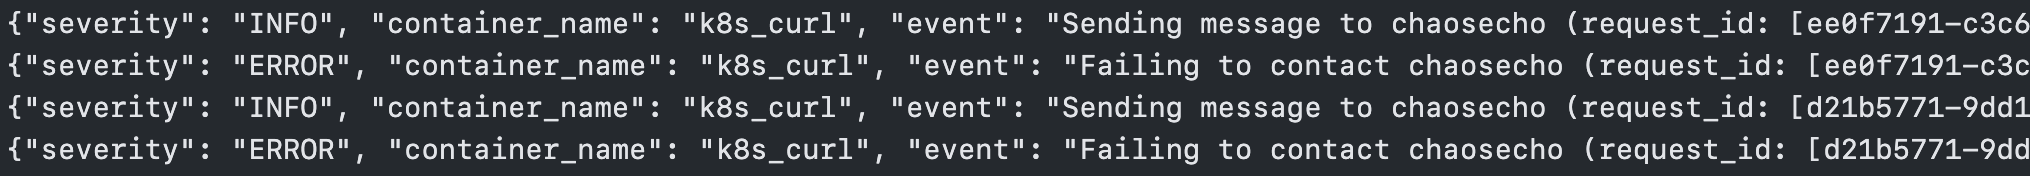
\includegraphics[width=\textwidth]{immagini/capitolo5/chaosecho_logs.png}
    \caption{Visualizzazione dei log.}
    \label{fig:chaosecho-logs}
\end{figure}

Eseguendo il deployment attraverso yRCA, e chiedendo di analizzare l'errore rilevato su \textit{curl}, si può notare quale sia stato il pod che ha causato il fallimento. Infatti, oltre ad essere presente l'errore \myenquote{\texttt{Error response (code: [Response Code]) received from...}}, il messaggio di output è composto da più linee, in quanto l'errore si è propagato \myenquote{a catena} fino ad arrivare a \textit{curl}. yRCA riesce quindi correttamente a ricostruire le interazioni, e a mostrare che a fallire è stato il pod \textit{backend}, in quanto l'ultimo messaggio che è stato inviato da \textit{middle} a \textit{backend} non ha ricevuto risposta, generando un errore di tipo  \myenquote{\texttt{Failing to contact [Service Name]]}}.


\begin{figure}[h]
    \centering
    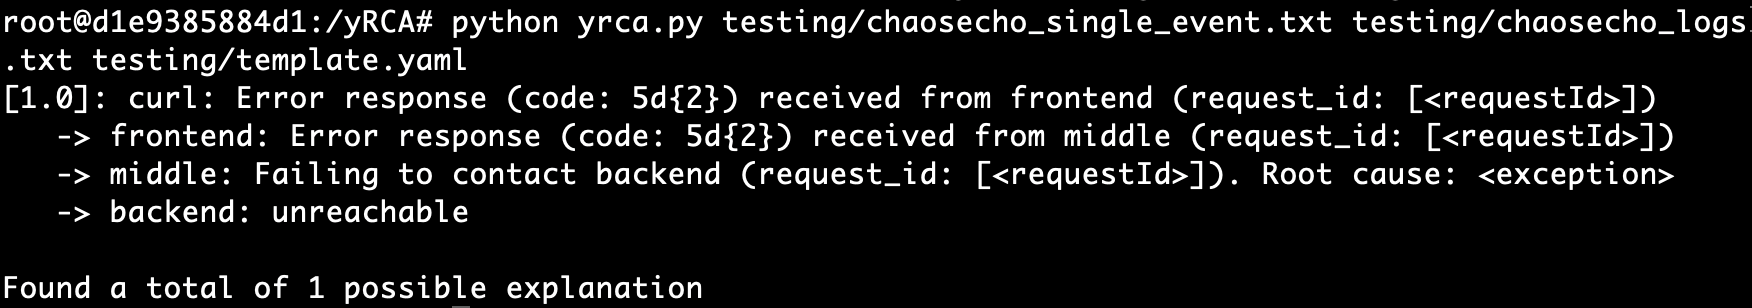
\includegraphics[width=\textwidth]{immagini/capitolo5/chaosecho_yrca.png}
    \caption{Visualizzazione dell'errore.}
    \label{fig:chaosecho-error}
\end{figure}

\section{Iniezione di un fallimento nell'applicazione Online Boutique} \label{sect:Iniezione di un fallimento nell'applicazione Online Boutique}

\subsection{Introduzione a Online Boutique}

Allo stesso modo di Istio con l'applicazione Bookinfo, altre piattaforme offrono applicazioni di esempio per aiutare gli sviluppatori. Una di queste applicazioni è \myenquote{Online Boutique}\footnote{https://github.com/GoogleCloudPlatform/microservices-demo} (o precedentemente conosciuta come \myenquote{Microservices Demo}), che rappresenta un moderno negozio online, funzionante tramite architettura a microservizi.

L'applicazione Online Boutique è composta da una serie di microservizi, tra cui:

\begin{itemize}
    \item \textit{Frontend:} Il front-end dell'applicazione, responsabile dell'interfaccia utente.
    \item \textit{Cart-service:} Gestisce il carrello della spesa dell'utente.
    \item \textit{Checkout-service:} Si occupa del processo di pagamento.
    \item \textit{Product-catalog-service:} Contiene il catalogo dei prodotti disponibili.
    \item \textit{Shipping-service:} Calcola i costi di spedizione.
    \item \textit{Payment-service:} Gestisce le transazioni di pagamento.
\end{itemize}

Per questo test, si vuole simulare un fallimento nel microservizio \textit{Payment-service}. Infatti, un fallimento in questo punto, non permette mai all'utente di completare l'acquisto, indipendentemente da quale articolo si vada ad acquistare. In particolare, si vuole creare un fallimento di tipo \myenquote{never started}, che si verifica quando il microservizio fallisce prima di generare log.

\subsection{Iniezione del fallimento}

Dopo aver eseguito lo script Python per modificare il deployment, ed averlo dispiegato correttamente nel cluster seguendo i passaggi illustrati per Bookinfo, si può procedere con la simulazione del fallimento simulando un blocco interno al container. Non appena viene creata la risorsa su Kubernetes, viene immediatamente portato a zero il numero di repliche del deployment \textit{payment-service}, per impedire ad esso di generare log. Ciò viene svolto tramite il comando presente nel Codice \ref{lst:paymentservice_zero}:
\begin{lstlisting}[caption={Configurazione del numero di repliche di \textit{payment-service.}}, label=lst:paymentservice_zero, language=bash]
    kubectl scale deployment paymentservice --replicas=0
\end{lstlisting}

Una volta generati i log con i metodi descritti al Capitolo \ref{sect:Iniezione di un fallimento nell'applicazione Bookinfo}, è possibile eseguire yRCA per ottenere il servizio che ha causato la serie di fallimenti a catena. Si chiede quindi a yRCA di ispezionare il log di errore del pod \textit{checkout-service}, essendo il pod che gestisce tutto il processo di acquisto \textit{(Figura \ref{fig:paymentservice_unreachable})}.

\begin{figure}[h]
    \centering
    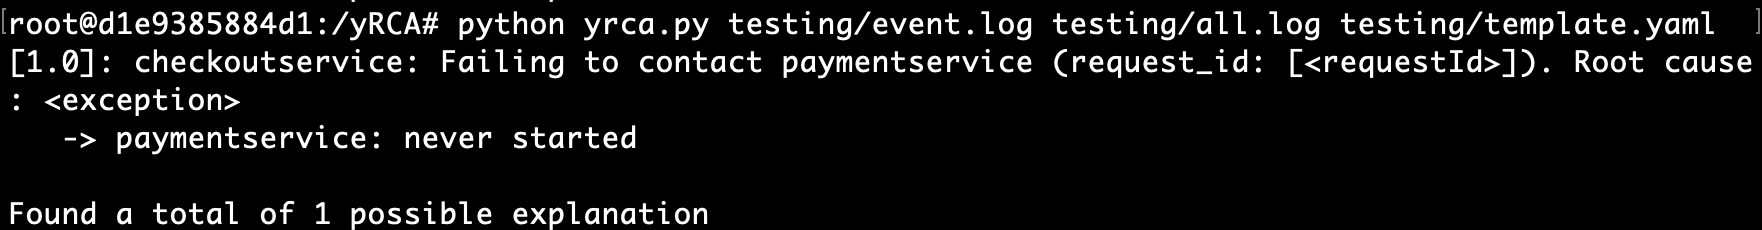
\includegraphics[width=\textwidth]{immagini/capitolo5/paymentservice_neverstarted.png}
    \caption{Analisi della causa di fallimento nell'applicazione Online Boutique.}
    \label{fig:paymentservice_unreachable}
\end{figure}

Dopo l'elaborazione, yRCA riporta correttamente la causa di errore, scoprendo che il pod a fallire è stato \textit{payment-service}, e che esso probabilmente non fosse mai stato avviato, non avendo mai generato log prima del fallimento.


\section{Iniezione di un fallimento nell'applicazione Sock Shop}

\subsection{Introduzione a Sock Shop}
Sock Shop\footnote{https://github.com/microservices-demo/microservices-demo} è un'applicazione demo a microservizi progettata per dimostrare il paradigma a microservizi in un e-commerce. Si tratta di un negozio online dove gli utenti possono visualizzare, cercare e acquistare calzini. L'applicazione utilizza diversi linguaggi e tecnologie per mostrare un approccio poli-tecnologico ai microservizi. 

L'architettura di Sock Shop comprende vari componenti, tra cui:

\begin{itemize}
    \item \textit{Front-End:} Interfaccia utente web del negozio.
    \item \textit{Catalogue:} Microservizio che gestisce l'inventario dei calzini disponibili.
    \item \textit{Cart:} Gestisce il carrello della spesa dell'utente.
    \item \textit{User:} Gestione degli utenti e delle sessioni di accesso.
    \item \textit{Orders:} Microservizio che gestisce gli ordini degli utenti.
    \item \textit{Shipping:} Si occupa delle spedizioni.
    \item \textit{Payment:} Gestione delle transazioni di pagamento.
\end{itemize}

Molti microservizi di questa applicazione hanno un database associato, che memorizza le informazioni persistenti relative alle funzionalità del microservizio. Ad esempio, il microservizio \myenquote{Catalogue} avrà un database che memorizza tutti i dettagli sui calzini disponibili, come nome, descrizione, prezzo e immagine. È possibile riconoscere ogni database dal microservizio associato, in quanto presenta una nomenclatura uguale a quest'ultimo, ma con il suffisso \texttt{-db}.

In Figura \ref{fig:sockshop-graph}, è osservabile un grafo dell'applicazione Sock Shop.

\begin{figure}[h]
    \centering
    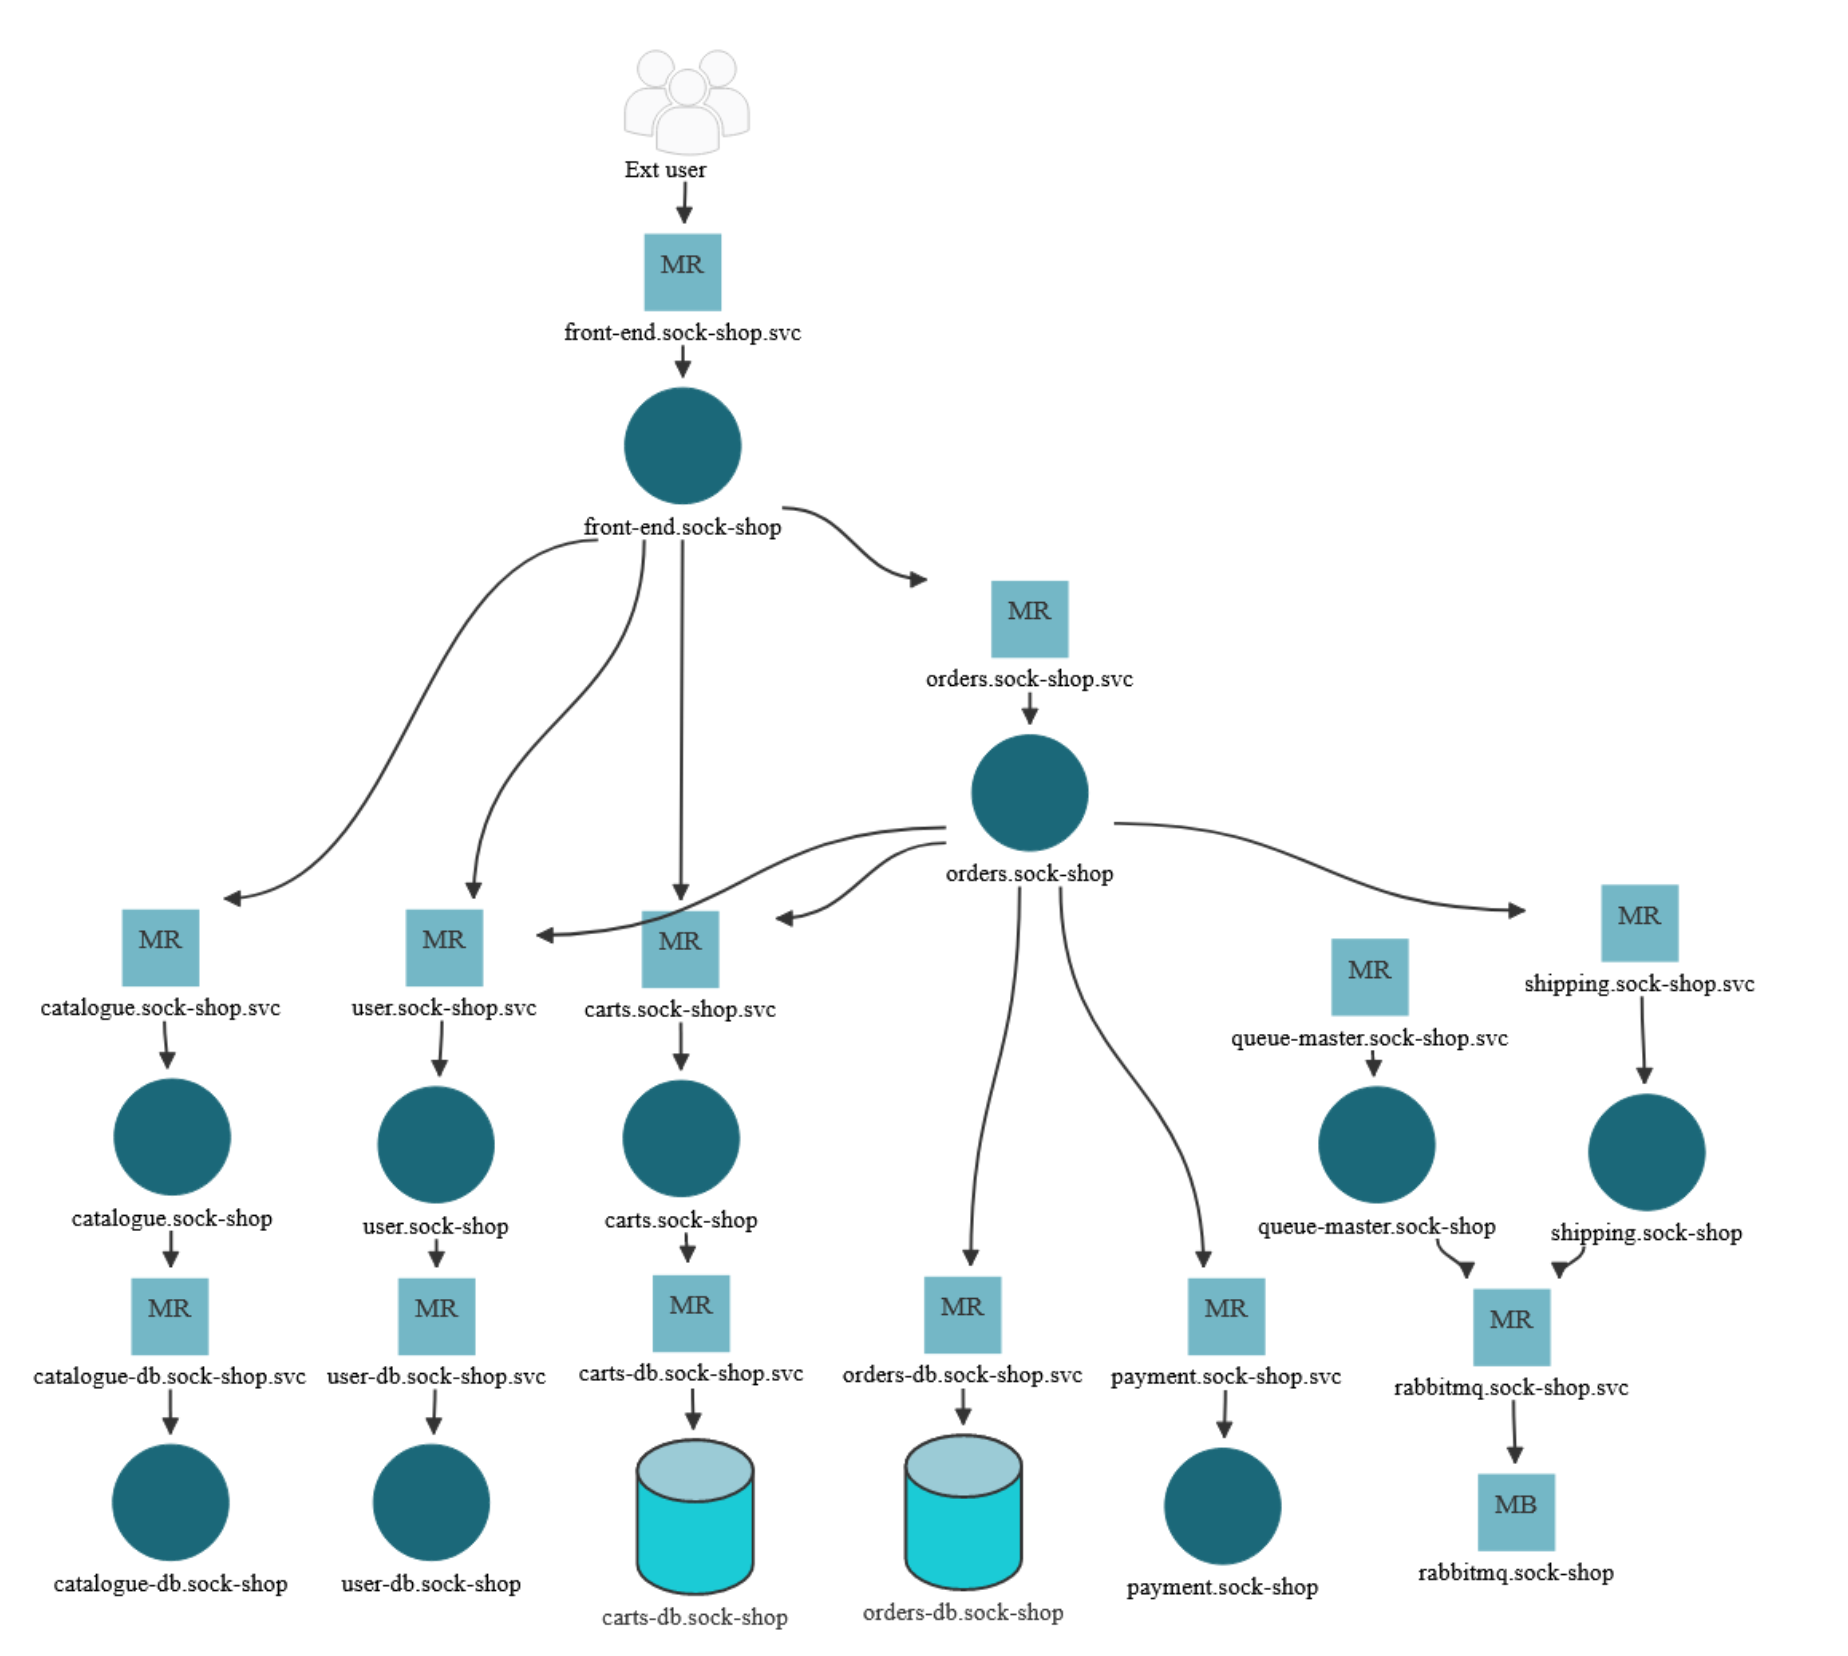
\includegraphics[width=\textwidth]{immagini/capitolo5/sockshop_graph.png}
    \caption{Grafo dell'applicazione a microservizi Sock Shop \cite{sockshop_graph}.}
    \label{fig:sockshop-graph}
\end{figure}

\subsection{Iniezione del fallimento}
Per testare il sistema con Sock Shop, verrà simulato un fallimento nel servizio \texttt{carts}. Il fallimento di questo componente rende impossibile l'aggiunta e la rimozione degli elementi dal carrello.

Anche in questo test, la preparazione dell'ambiente relativa al dispiegamento del deployment di Sock Shop modificato è identica a quella vista per gli altri test. Dopo aver sospeso l'esecuzione di \texttt{carts}, il sito è rimasto ancora completamente visitabile e navigabile, ma aggiungere prodotti al carrello non sembrava avere effetto dall'interfaccia browser, e ispezionando l'errore utilizzando la console di sviluppo del browser, è stato possibile notare l'errore riportato in Figura \ref{fig:sockshop-error}.

\begin{figure}[h]
    \centering
    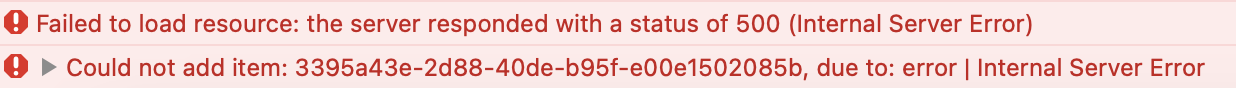
\includegraphics[width=\textwidth]{immagini/capitolo5/browser_error.png}
    \caption{Errore nella console browser.}
    \label{fig:sockshop-error}
\end{figure}

Come effettuato per i test precedenti, è stato possibile analizzare il fallimento con yRCA, consentendo quindi di scoprire quale sia stato il pod a causare i fallimenti \textit{(Figura \ref{fig:sockshop-yrca})}.

\begin{figure}[h]
    \centering
    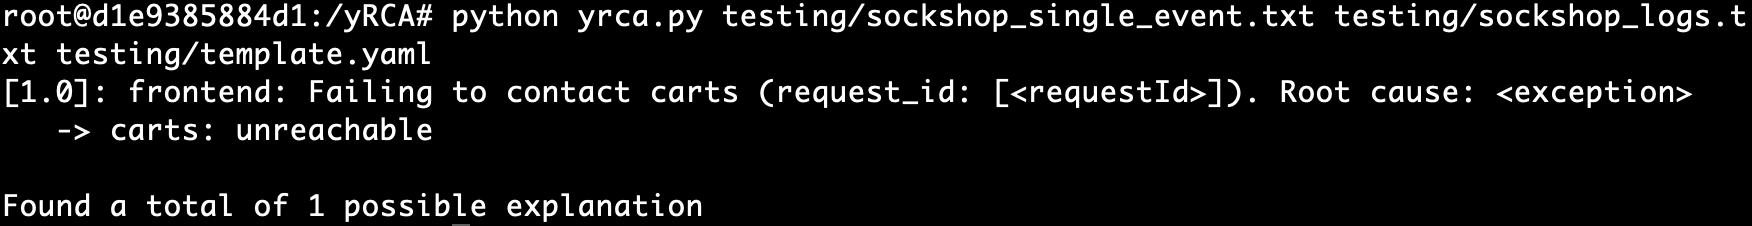
\includegraphics[width=\textwidth]{immagini/capitolo5/new_sockshop_yrca.png}
    \caption{Spiegazione del fallimento nell'applicazione Sock Shop.}
    \label{fig:sockshop-yrca}
\end{figure}

\section{Analisi delle prestazioni}
\subsection{Introduzione}
Un aspetto importante relativo alla validazione della soluzione è analizzare che la stessa abbia sul cluster un impatto prestazionale accettabile e generalmente proporzionato alla complessità dell'ambiente che si vuole monitorare. È infatti necessario che la soluzione proposta non introduca un \textit{overhead}, tale da far sì che i benefici derivati dall'implementazione della soluzione proposta non siano giustificati dal costo che la stessa soluzione ha in termini di risorse.

Per l'analisi delle prestazioni, sono state considerate le seguenti metriche:

\begin{itemize}
    \item \textbf{Utilizzo CPU e RAM:} metriche per misurare l'overhead della soluzione in termini di utilizzo di CPU e memoria RAM. È importante notare che su Kubernetes l'unità di misura per il consumo della CPU è il \myenquote{core}, che rappresenta un'unità logica del processore. Questo valore indica quanta capacità di elaborazione CPU un'applicazione o servizio sta utilizzando all'interno di un pod.
    \item \textbf{Utilizzo delle immagini:} metrica che misura lo spazio occupato da tutte immagini Docker dai componenti della soluzione.
    \item \textbf{Tempi di latenza:} metrica per misurare la variazione del tempo di risposta di un'applicazione a microservizi quando la soluzione viene applicata. 

\end{itemize}

Tutti i test sono stati svolti su Minikube in esecuzione su un ambiente Docker, con 8 GB di RAM e 8 threads CPU dedicati.

\subsection{Analisi di CPU e RAM}
Per lo scopo di questo test, sono stati posti sotto test tre dei quattro dispiegamenti trattati nel Capitolo \ref{chap:Validazione della soluzione}. È stato infatti deciso di analizzare l'utilizzo CPU e RAM nei deployment di applicazioni realistiche, ovvero:
\begin{itemize}
    \item \textit{Online Boutique}
    \item \textit{Bookinfo}
    \item \textit{Sock Shop}
\end{itemize}

Per monitorare l'utilizzo di CPU e RAM della soluzione, è necessario in primis installare il \textit{Metrics Server}\footnote{https://github.com/kubernetes-sigs/metrics-server}, un componente che consente di ottenere i dati relativi alle metriche sulle prestazioni dai Kubelet, per poi esporle all'API Server tramite le \textit{Metrics API}. Quest'ultime sono poi accessibili tramite il comando presente nel Codice \ref{lst:kubectl-metrics}:
\begin{lstlisting}[caption={Comando per la rilevazione di metriche.}, label=lst:kubectl-metrics, language=bash]
    kubectl top pods -n <nome del namespace da monitorare>
\end{lstlisting}

Per ottenere una percentuale di overhead, è necessario ottenere il consumo di CPU e RAM per un dispiegamento con funzionalità di raccolta del logging, e compararlo allo stesso deployment, ma senza le suddette funzionalità abilitate.

Nella Tabella \ref{table:cpu_analysis}, è possibile notare l'utilizzo di CPU e RAM del dispiegamento Online Boutique, con le funzioni di logging abilitate. Tali metriche sono state rilevate più volte, nell'arco di 5 minuti, mentre verso il cluster viaggiava un traffico costante di richieste GET. I valori non si sono mai discostati in modo significativo da quelli riportati in Tabella \ref{table:cpu_analysis}.

\begin{table}[h]
\centering
\begin{tabular}{|l|l|c|c|c|}
\hline
\rowcolor{lightgray}
\textbf{Applicazione} & \textbf{Tipo} & \textbf{CPU (m)} & \textbf{RAM (MB)} & \textbf{Overhead \%} \\
\hline
\multirow{2}{*}{Online-Boutique} & Base & 181m & 586 MB & \multirow{2}{*}{CPU: 131.49\%, RAM: 646.42\%} \\
& Con logging & 419m & 4374 MB & \\
\hline
\multirow{2}{*}{Bookinfo} & Base & 197m & 760 MB & \multirow{2}{*}{CPU: 170.56\%, RAM: 441.32\%} \\
& Con logging & 533m & 4114 MB & \\
\hline
\multirow{2}{*}{Sock Shop} & Base & 161m & 2825 MB & \multirow{2}{*}{CPU: 463.35\%, RAM: 128.96\%} \\
& Con logging & 907m & 6468 MB & \\
\hline
\end{tabular}
\caption{Confronto dell'utilizzo delle risorse per i tipi di dispiegamento.}
\label{table:cpu_analysis}
\end{table}

Per il dispiegamento Online Boutique, si dà in Figura \ref{fig:perf_analysis} anche un dettaglio dell'utilizzo CPU e RAM tra i pod dei vari namespace.

\begin{figure}[h]
    \centering
    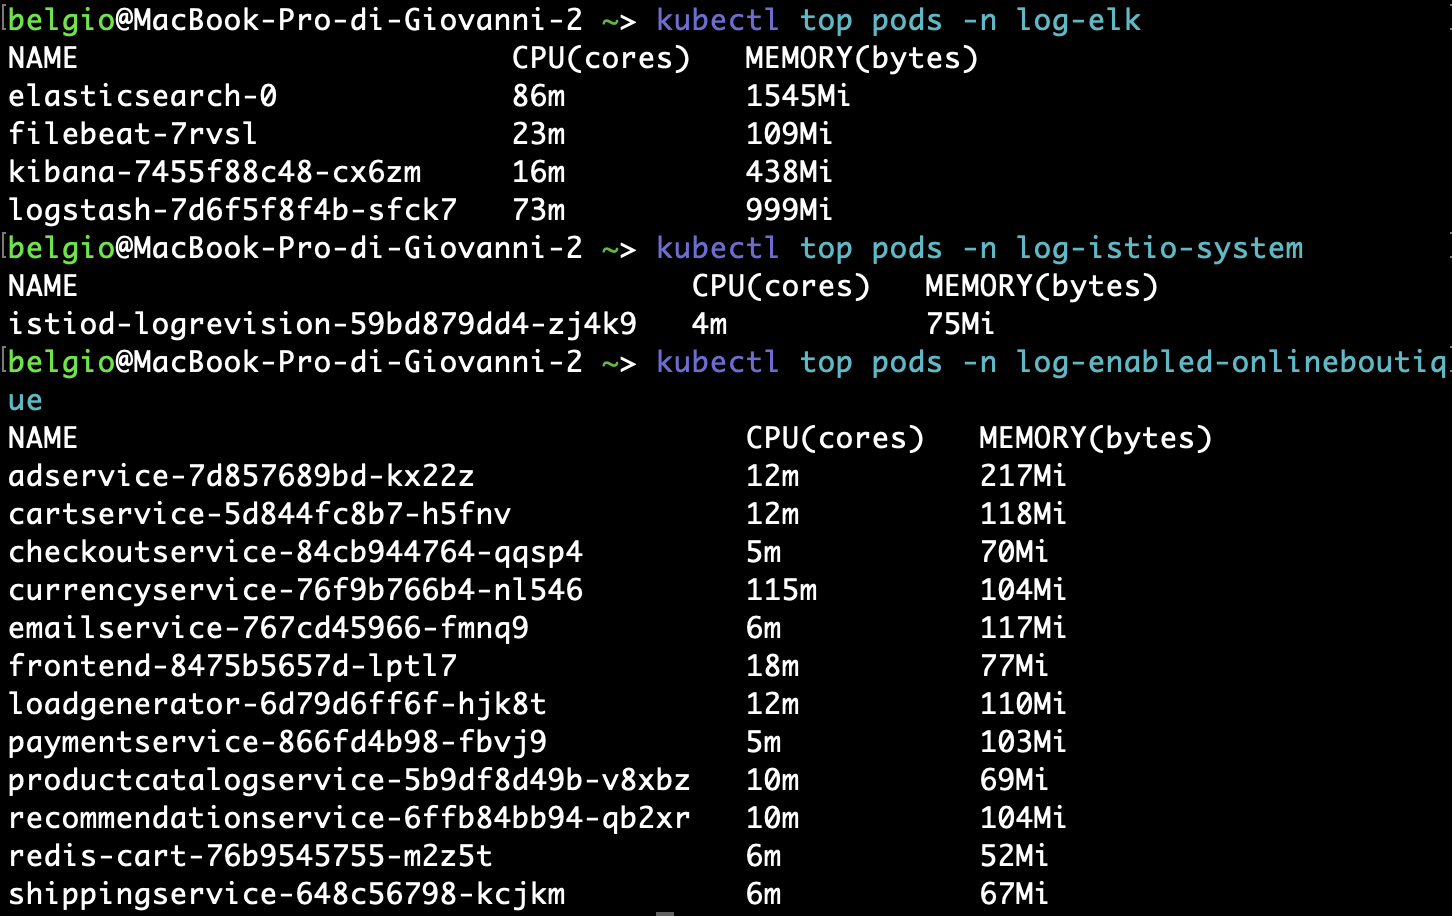
\includegraphics[width=\textwidth]{immagini/capitolo5/cpu_onlineboutique.png}
    \caption{Visualizzazione del consumo di CPU e RAM dei singoli componenti per il dispiegamento Online Boutique.}
    \label{fig:perf_analysis}
\end{figure}

\subsection{Analisi dell'utilizzo di storage delle immagini}
Per procedere all'analisi delle metriche sull'utilizzo dello storage, viene usato il supporto Docker integrato a Minikube, descritto nel Capitolo \ref{Iniezione del fallimento}. Una volta attivato, è possibile tramite vedere l'utilizzo di tutte le immagini presenti nel cluster tramite il comando:
\begin{lstlisting}
    docker images
\end{lstlisting}
Per questo test, i dati riportati per lo storage sono presenti nella Tabella \ref{tab:storage_usage}.
\begin{table}[H]
    \centering
    \begin{tabular}{|c|c|}
    \hline
    \rowcolor{lightgray}
        Nome immagine & Utilizzo \\ \hline
       Istiod  &  167 MB \\ \hline
       Proxy Envoy & 241 MB\\ \hline
       ElasticSearch  & 837 MB\\ \hline
       Logstash & 1,68 GB\\ \hline
       Kibana & 1,27 GB\\ \hline
       Filebeat & 1,16 GB\\ \hline
      \rowcolor{lightgray}
      Totale & 5,35 GB \\ \hline
    \end{tabular}
    \caption{Tabella sull'utilizzo dell'archiviazione.}
    \label{tab:storage_usage}
\end{table}
Come è possibile rilevare, la maggior parte dell'archiviazione è occupata dai componenti dello stack ELK, in quanto trattasi di servizi complessi, con un grande numero di funzionalità, e che necessitano di svariate dipendenze e librerie. Al contrario, è stato rilevato che Istio e i Proxy Envoy utilizzano una quantità molto minore di archiviazione, con una somma che arriva a 408 MB di spazio utilizzato.

La Tabella \ref{table:storage_comparison} mostra invece quanto vadano ad incidere, in termini  assoluti e percentuali, le componenti di Istio e dello stack ELK sullo spazio di archiviazione complessivo per ciascuna applicazione.

\begin{table}[h]
\centering
\begin{tabular}{|l|c|c|c|}
\hline
\rowcolor{lightgray}
\textbf{Applicazione} & \textbf{Base} & \textbf{Con logging} & \textbf{Overhead (\%)} \\
\hline
Bookinfo & 2377 MB & 7732 MB & 225.28 \% \\
\hline
Online Boutique & 1712,2 MB & 7067,2 MB & 312,76 \% \\
\hline
Sock Shop & 2991,4 MB & 8346,4 MB & 179,01 \% \\
\hline
\end{tabular}
\caption{Overhead per l'archiviazione nelle varie applicazioni di test.}
\label{table:storage_comparison}
\end{table}




\subsection{Analisi della latenza}
L'ultima metrica oggetto di analisi è stata la latenza. In particolare, si è voluto analizzare quanto la soluzione proposta impattasse i tempi delle interazioni tra i pod del cluster. A differenza delle metriche misurate nei capitoli precedenti, dove l'overhead è direttamente proporzionale al numero di container o risorse utilizzate, l'overhead per i tempi di latenza dipende maggiormente dal numero di interazioni scambiate tra i pod. La causa di questo overhead è potenzialmente attribuibile al proxy Envoy, che agendo da componente che intercetta ogni chiamata tra i pod, introduce un quantitativo di latenza in ogni comunicazione. Per comprendere se ciò potesse impattare in modo significativo, è stato fondamentale analizzare e confrontare la latenza tra le richieste effettuate in un ambiente con e senza la soluzione proposta. È stato quindi sviluppato uno script \textit{Bash} in grado di eseguire i test oggetto di analisi. Tale script si avvale dello strumento di benchmarking \texttt{wrk}\footnote{https://github.com/wg/wrk} per generare carichi di lavoro e misurare la latenza delle richieste HTTP. Le sperimentazioni sono state condotte simulando diversi scenari d'uso, variando il numero di connessioni contemporanee (per simulare un numero variabile di potenziali utenti), e dispiegando i componenti singolarmente, per misurare l'impatto di ognuno sul sistema. 
In particolare, i test sono stati effettuati con:
\begin{itemize}
    \item \textbf{Deployment base:} Il dispiegamento originale, senza la soluzione applicata.
    \item \textbf{Deployment con Istio:} Il dispiegamento base, con in aggiunta solo i componenti di Istio.
    \item \textbf{Deployment con Istio + ELK:} Il dispiegamento con tutti i componenti della soluzione proposta.
\end{itemize}
Lo script Bash è composto dai seguenti passi:
\begin{enumerate}
    \item \textbf{Applicazione del deployment:} Viene applicato al cluster il deployment di test tramite il comando \texttt{kubectl apply}.
    \item \textbf{Attesa:} Vengono attesi 120 secondi tra l'applicazione delle risorse e l'inizio del testing, in modo da attendere che tutte le risorse siano dispiegate ed avviate correttamente.
    \item \textbf{Test:} Viene eseguito \texttt{wrk}, configurato per essere eseguito più volte, variando tra di loro il numero di connessioni da tenere attive contemporaneamente. In particolare, i test sono stati svolti con 8, 25, 50 e 200 connessioni contemporanee aperte, per simulare più casi d'uso. Tutti i test vengono eseguiti con un tempo limite fissato a 60 secondi.
    \item \textbf{Rimozione del deployment:} Il deployment testato viene rimosso dal cluster, in modo tale da poter eventualmente eseguire nuovamente lo script con un altro deployment senza creare interferenze.
    \item \textbf{Output dei dati:} Lo script restituisce l'output di \texttt{wrk} su un file, il quale nome è specificato come parametro di input.
\end{enumerate}
Come dispiegamento di test, è stato scelto Bookinfo, in quanto trattasi di un'applicazione con una struttura semplice e già trattata nella tesi al Capitolo \ref{sect:Iniezione di un fallimento nell'applicazione Bookinfo}, ma che coinvolge comunque diverse interazioni tra microservizi in una singola chiamata HTTP GET.

Nella Tabella \ref{table:tabella_latenze}, è possibile vedere il risultato dei test effettuati sull'ambiente Bookinfo.


\begin{table}[h]
\centering
\begin{tabular}{|c|c|c|c|c|c|}
\hline
\rowcolor{lightgray}
\textbf{Utenti} & \textbf{Deployment} & \textbf{Latenza AVG} & \textbf{Latenza Stdev} & \textbf{Richieste/sec} & \textbf{Overhead \%} \\
\hline
\multirow{3}{*}{8} & Base & 34.62ms & 28.64ms & 248.26 & - \\
& con Istio & 63.18ms & 37.09ms & 130.31 & 82.5\% \\
& con Istio + ELK & 67.32ms & 40.92ms & 122.92 & 94.4\% \\
\hline
\multirow{3}{*}{25} & Base & 97.70ms & 45.11ms & 252.60 & - \\
& con Istio & 101.06ms & 45.84ms & 243.37 & 3.44 \% \\
& con Istio + ELK & 108.07ms & 28.55ms & 221.85 & 10.6 \% \\
\hline
\multirow{3}{*}{50} & Base & 180.12ms & 24.49ms & 265.55 & - \\
& con Istio & 191.75ms & 22.38ms & 249.79 & 6.5\% \\
& con Istio + ELK & 219.20ms & 35.49ms & 218.59 & 21.7\% \\
\hline
\multirow{3}{*}{200} & Base & 784.47ms & 91.08ms & 253.53 & - \\
& con Istio & 829.61ms & 57.54ms & 239.13 & 5.8\% \\
& con Istio + ELK & 941.63ms & 107.88ms & 210.67 & 20.0\% \\
\hline
\end{tabular}
\caption{Misurazioni rilevate nell'ambiente Bookinfo.}
\label{table:tabella_latenze}
\end{table}




Come è possibile notare, la latenza aumenta proporzionalmente all'aumentare del numero di utenti che interagiscono con l'applicazione. Questo comportamento è atteso, dato che un maggior numero di richieste mette sotto stress il sistema e può portare, come in questo caso, a ritardi nella risposta. Anche la presenza di Istio e ELK influisce sul tempo di risposta, con una latenza che tende ad aumentare in presenza di questi strumenti rispetto al deployment base. Ciò è in linea con quanto atteso, visto che l'introduzione di proxy come Envoy e l'overhead aggiuntivo introdotto dallo stack ELK per la raccolta di log possono anch'essi aggiungere ritardi nelle comunicazioni.

In particolare, si nota che:
\begin{itemize}
\item Con carico pari a 8 utenti, il deployment con Istio presenta una latenza media di circa 30ms in più rispetto al deployment base. Questo test, effettuato unicamente per completezza, non risulta però essere di particolare rilevanza, vista l'alta variabilità dei dati (dato rilevato dalla deviazione standard), che porta ad un'altissima percentuale di overhead. Questa variabilità è probabilmente dovuta al port forwarding che Minikube, in esecuzione su Docker, esegue per rendere disponibili i servizi al sistema host \cite{ibm_report_docker}.
\item Al crescere degli utenti, i dati diventano sempre man mano più consistenti, ed è possibile ottenere delle stime sempre più precise. L'overhead introdotto dallo stack ELK si attesta circa al 20\%, mentre quello relativo ad Istio è di pochi punti percentuale.
\item Sono stati svolti test anche con un numero superiore di connessioni (500 e 1000), ma questi test non hanno riportato nessuna informazione utile, perché l'ingente numero di connessioni ha portato al sovraccarico dell'ambiente di test, risultando nella quasi totalità delle risposte in timeout.
\end{itemize}

È importante menzionare che questi test sono stati eseguiti con l'unico scopo di ottenere un'idea generale dell'incremento di latenza con l'aggiunta della soluzione proposta, ma possono non rispecchiare veri casi d'uso in un cluster. Infatti, i test sono stati condotti in un ambiente Minikube, che rappresenta un ambiente di sviluppo locale e su nodo singolo per Kubernetes. L'hardware, la configurazione e i limiti imposti da Minikube non sono rappresentativi di un vero ambiente di produzione. Pertanto, i risultati ottenuti possono variare significativamente quando la soluzione proposta viene applicata in un vero cluster Kubernetes su un'infrastruttura adeguata.
\chapter{Conclusioni}
L'obiettivo della tesi posto all'inizio della relazione era automatizzare il logging delle interazioni in un ambiente Kubernetes, al fine di identificare le cause principali dei malfunzionamenti nei deployment. In questo documento, si è mostrata una possibile soluzione che non necessita di modificare il codice delle applicazioni. Per quanto riguarda i contributi descritti al Capitolo 1, è stata inizialmente sviluppata una metodologia che, tramite la simbiosi di più componenti, è in grado di fornire il logging delle interazioni, partendo da un file di deployment esistente. Nell'implementazione, è stato poi fornito un programma Python che dimostra come questa configurazione possa essere realizzata automaticamente. Si è poi proceduto alla fase di testing, dove l'implementazione corrente è stata testata con applicazioni di benchmarking esistenti, quali Bookinfo, Chaos Echo, Online Boutique e Sock Shop, simulando multipli tipi di fallimenti.

Allo stadio attuale, sono presenti limitazioni che potrebbero essere affrontate in futuro, sia riguardanti la metodologia, sia riguardanti l'implementazione del prototipo. Parlando della metodologia, è necessaria una sperimentazione più accurata ed estensiva, valutando il comportamento del prototipo su diverse architetture Kubernetes, e con dispiegamenti realmente utilizzati in ambienti di produzione. Questo permetterebbe di validare il prototipo in ambienti reali, dove le variabili e le dinamiche sono molteplici, e potrebbero differire di molto da quelle dei benchmark utilizzati. Inoltre, per quanto concerne la sicurezza, la metodologia proposta presenta alcuni problemi, in particolare per quanto riguarda l'ottenimento dei log. Sarebbe infatti necessario sia un sistema di autenticazione verso l'istanza ElasticSearch, in quanto il servizio attualmente non ne prevede alcuna, rendendo quindi possibile a tutti l'ottenimento dei log se il servizio venisse erroneamente esposto ad Internet. Anche la comunicazione con l'istanza ElasticSearch avviene in chiaro, rendendo non sicuro il trasferimento delle informazioni tramite Internet. Infine, per quanto riguarda l'utilizzo, la soluzione richiede comunque un'attenzione manuale per la parte riguardante l'accesso al pod con l'istanza ElasticSearch, che in un normale ambiente Kubernetes richiede una configurazione manuale sia del punto di Ingress, sia di eventuali firewall in esecuzione sul sistema. Per aggirare questa limitazione, tutta l'elaborazione dello script Python e il post-processing potrebbero essere affrontati in un container Docker in esecuzione sullo stesso namespace, e restituendo su \verb|stdout| direttamente l'output finale di yRCA.

Per quanto riguarda il prototipo, questo potrebbe essere poi ulteriormente esteso con capacità di esportazione del file di output maggiori, come ad esempio la scrittura su un bucket cloud, o l'integrazione con piattaforme di monitoraggio come Grafana\footnote{https://grafana.com} o Prometheus\footnote{https://prometheus.io}. Questo permetterebbe una visualizzazione immediata e interattiva dei dati raccolti, favorendo una diagnosi più rapida e accurata dei problemi riscontrati nelle applicazioni.

\bibliographystyle{plainurl} % We choose the "plain" reference style
\bibliography{bibliography}
%\addbibresource{bibliography.bib}
%\printbibliography

\end{document}
